%%%%%%%%%%%%%%%%%%%%%%%%%%%%%%%%%%%%%%%%%%%%%%%%%%%%%%%%%%%%%%%%%%%%%%%%%%%%%%%%%%
\begin{frame}[fragile]\frametitle{}
\begin{center}
{\Large Machine Learning Concepts}
\end{center}
\end{frame}

%%%%%%%%%%%%%%%%%%%%%%%%%%%%%%%%%%%%%%%%%%%%%%%%%%%%%%%%%%%%%%%%%%%%%%%%%%%%%%%%%%
\begin{frame}[fragile]\frametitle{}
\begin{center}
{\Large Machine Learning way of Solution, Mathematically}
\end{center}
\end{frame}


%%%%%%%%%%%%%%%%%%%%%%%%%%%%%%%%%%%%%%%%%%%%%%%%%%%%%%%%%
\begin{frame}[fragile]\frametitle{General Form}
$Y= F(X_1, X_2,\ldots, X_p)$
\begin{itemize}
\item We have:
	\begin{itemize}
	\item Observation of quantitative (numerical) response $Y$
	\item Observation of $p$ different predictors ${X_1, X_2, \ldots, X_p}$
	\end{itemize}
	\item Find function $F$ between $Y$ and $X = {X_1, X_2,\ldots, X_p}$
\end{itemize}
\end{frame}

%%%%%%%%%%%%%%%%%%%%%%%%%%%%%%%%%%%%%%%%%%%%%%%%%%%%%%%%%
\begin{frame}[fragile]\frametitle{General Form}
As one may not get exact function $F$, approximate it to $f$, thus introducing some error.
\begin{itemize}
\item So, general form: $Y = f(X) + \epsilon$
\item $f$ is unknown function of ${X_1, X_2, \ldots, X_p}$
\item  $\epsilon$ is a random error term, Independent of X, Has mean equal to zero
% \item $f$ represents information that $X$ provides about $Y$
\item Statistical learning refers to approaches for estimating $f$
\end{itemize}
\end{frame}



%%%%%%%%%%%%%%%%%%%%%%%%%%%%%%%%%%%%%%%%%%%%%%%%%%%%%%%%%%
\begin{frame}[fragile]\frametitle{Estimate $f$}
\begin{itemize}
\item Not concerned if $f$ is linear, quadratic, etc.
\item We only care that our predictions are ``near accurate''.
\item So, $f$ often treated as a black box. 
\item The aim is of minimizing reducible error
% \item The irreducible error will always provide an upper bound on the accuracy of our predictions.
\end{itemize}
\end{frame}


%%%%%%%%%%%%%%%%%%%%%%%%%%%%%%%%%%%%%%%%%%%%%%%%%%%%%%%%%
\begin{frame}[fragile]\frametitle{How do we estimate $f$?}
Most statistical learning methods classified as:
	\begin{itemize}
	\item Parametric
	\item Non-parametric
	\end{itemize}
\end{frame}

%%%%%%%%%%%%%%%%%%%%%%%%%%%%%%%%%%%%%%%%%%%%%%%%%%%%%%%%%
\begin{frame}[fragile]\frametitle{How do we estimate $f$?}
\begin{itemize}
\item Parametric:
	\begin{itemize}
	\item Assume that the functional form, or shape, of $f$ in linear in $X$, $f(X) = \sum_{i=1}^p \beta_i X_i$
	\item This is a linear model, for $p$ predictors $X = {X_1, X_2,\ldots, X_p}$
	\item Model fitting involves estimating the parameters $\beta_0, \beta_1,\ldots,\beta_p$
	\item Reduces the problem of estimating $f$ to estimating a set of parameters
	\end{itemize}
\item Non-Parametric: No explicit assumptions about the functional form of $f$
\end{itemize}
\end{frame}

%%%%%%%%%%%%%%%%%%%%%%%%%%%%%%%%%%%%%%%%%%%%%%%%%%%
\begin{frame}[fragile] \frametitle{Comparison}

\adjustbox{valign=t}{
\begin{minipage}{0.45\linewidth}
Parametric
\begin{itemize}
\item Only need to estimate set of parameters
\item Bias such as linear model
\item May not fit data well
\end{itemize}

\end{minipage}
}
\hfill
\adjustbox{valign=t}{
\begin{minipage}{0.45\linewidth}
Non-Paremetric
\begin{itemize}
\item Potential of many shapes for $f$
\item Lots of observations needed
\item Complex models can overfit
\end{itemize}

\end{minipage}
}
\end{frame}

%%%%%%%%%%%%%%%%%%%%%%%%%%%%%%%%%%%%%%%%%%%%%%%%%%%%%%%%%
\begin{frame}[fragile]\frametitle{Simple Example}
\begin{itemize}
\item Linear regression is a simple and useful tool for predicting
a quantitative response. The relationship between input
variables $X = (X_1 , X_2 , \ldots X_p )$ and output variable $Y$ takes
the form: $Y \approx \beta_0 + \beta_1 X_1 + \ldots + \beta_p X_p + \epsilon$
\item $\beta_0 , \beta_1 ,\ldots \beta_p$ are the unknown coefficients (parameters) which
we are trying to determine. 
\item The best coefficients will lead us to the best ``fit'', which can be found by
minimizing the residual sum squares (RSS), or the sum of the difference between the actual $i$th value and
the predicted $i$th value. 
\item $RSS = \sum_{i=1}^n = e_i$ , where $e_i = y_i - y'$
\end{itemize}
\end{frame}

%%%%%%%%%%%%%%%%%%%%%%%%%%%%%%%%%%%%%%%%%%%%%%%%%%%%%%%%%
\begin{frame}[fragile]\frametitle{How to find best fit?}
Matrix Form:
\begin{itemize}
\item  We can solve the closed-form equation for coefficient vector $w$: $w = (X^T X^{-1}) X^T Y$. 
\item $X$ represents the input data and $Y$ represents the output data. 
\item This method is used for smaller matrices, since inverting a matrix is computationally expensive.
\end{itemize}
\end{frame}

%%%%%%%%%%%%%%%%%%%%%%%%%%%%%%%%%%%%%%%%%%%%%%%%%%%%%%%%%
\begin{frame}[fragile]\frametitle{How to find best fit?}
Gradient Descent:
\begin{itemize}
\item First-order optimization algorithm.
\item We can find the minimum of a convex function by
starting at an arbitrary point and repeatedly take steps
in the downward direction, which can be found by taking
the negative direction of the gradient. 
\item After several
iterations, we will eventually converge to the minimum.
In our case, the minimum corresponds to the coefficients
with the minimum error, or the best line of fit. 
\item The
learning rate $\alpha$ determines the size of the steps we take
in the downward direction.
\end{itemize}
\end{frame}

%%%%%%%%%%%%%%%%%%%%%%%%%%%%%%%%%%%%%%%%%%%%%%%%%%%%%%%%%
\begin{frame}[fragile]\frametitle{How to find best fit?}
Gradient descent algorithm in two dimensions (meaning with 2 features, as example):
\begin{itemize}
\item  Repeat until convergence.
\begin{align*}
w_0^{t+1} &= w_0^t - \alpha \frac{\partial J(w_0,w_1)}{\partial w_{0}}\\
w_1^{t+1} &= w_1^t - \alpha \frac{\partial J(w_0,w_1)}{\partial w_{1}}
\end{align*}
\item For non convex functions, gradient descent no longer guarantees an optimal solutions since there may be local minimas. 
\item Instead, we should run the algorithm from different
starting points and use the best local minima we find for
the solution.
\end{itemize}

\end{frame}

%%%%%%%%%%%%%%%%%%%%%%%%%%%%%%%%%%%%%%%%%%%%%%%%%%%%%%%%%
\begin{frame}[fragile]\frametitle{How to find best fit?}
Stochastic Gradient Descent:

\begin{itemize}
\item  Instead of taking a step
after sampling the entire training set, we take a small
batch of training data at random to determine our next
step. 
\item Computationally more efficient and may lead to
faster convergence.
\end{itemize}

\end{frame}

% %%%%%%%%%%%%%%%%%%%%%%%%%%%%%%%%%%%%%%%%%%%%%%%%%%%%%%%%%%
% \begin{frame}[fragile]\frametitle{Machine Learning }
% \begin{center}
% 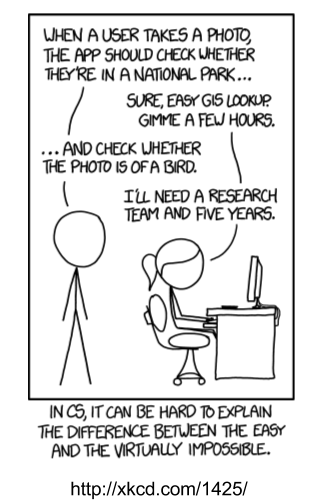
\includegraphics[width=0.35\linewidth,keepaspectratio]{mlxkcd}
% \end{center}
% \tiny{(Reference: https://blog.algorithmia.com/wp-content/uploads/2016/10/Intro-to-Machine-Learning-e1477946721913.png)}
% \end{frame}


%%%%%%%%%%%%%%%%%%%%%%%%%%%%%%%%%%%%%%%%%%%%%%%%%%%%%%%%%%%%
%%\begin{frame}[fragile]\frametitle{Hypothesis}
%%\begin{center}
%%{\em ``A fact is a simple statement that everyone believes. It is innocent, unless found guilty. A hypothesis is a novel suggestion that no one wants to believe. It is guilty, until found effective''}
%%\end{center}
%%- Edward Teller, the famous Hungarian-American physicist
%%\end{frame}


%%%%%%%%%%%%%%%%%%%%%%%%%%%%%%%%%%%%%%%%%%%%%%%%%%%%%%%%%%%%%
%%\begin{frame}[fragile]\frametitle{Hypothesis Testing}
%%\begin{itemize}
%%\item Make Assumptions.
%%\item Take an initial position.
%%\item Determine the alternate position.
%%\item Set acceptance criteria
%%\item Conduct fact based tests.
%%\item Evaluate results. Does the evaluation support the initial position? Are we confident that the result is not due to chance?
%%\item Reach one of the following conclusion: Reject the original position in favor of alternate position or fail to reject the initial position.
%%\end{itemize}
%%
%%\end{frame}
%%
%%%%%%%%%%%%%%%%%%%%%%%%%%%%%%%%%%%%%%%%%%%%%%%%%%%%%%%%%%%%%
%%\begin{frame}[fragile]\frametitle{The NULL Hypothesis (Ho)}
%%\begin{itemize}
%%\item The null hypothesis is the initial position. 
%%\item It is the status-quo position. 
%%\item It is the position that is rejected or fails to be rejected. 
%%\item It is the position that needs to be validated. 
%%\item It is the position that needs to be tested.
%%\item Hypothesis: More you study you will get more marks.
%%\item Null Hypothesis: More study does NOT have any effect on marks.
%%\item Whole idea is to disprove Null Hypothesis to prove your Hypothesis.
%%\item Thus, one has to show there is no RELATIONSHIP between two, ie no fitting line exists. Its Random.
%%\end{itemize}
%%
%%\end{frame}

%%%%%%%%%%%%%%%%%%%%%%%%%%%%%%%%%%%%%%%%%%%%%%%%%%%%%%%%%%%%%%%%%%%%%%%%%%%%%%%%%%
\begin{frame}[fragile]\frametitle{}
\begin{center}
{\Large Cross Validation}
\end{center}
\end{frame}


%%%%%%%%%%%%%%%%%%%%%%%%%%%%%%%%%%%%%%%%%%%%%%%%%%%%%%%%%%
\begin{frame}[fragile]\frametitle{Background: Imp Terms}

	\begin{itemize}
	\item {\bf Learning algorithm:} identifies a model that best fits the relationships between inputs and outputs. 
	\item {\bf Training set:} consists of records with features and with/without class labels 
	\item {\bf Test set:} consists of records with only features, class labels to be computed.
	\end{itemize}
\end{frame}


%%%%%%%%%%%%%%%%%%%%%%%%%%%%%%%%%%%%%%%%%%%%%%%%%%%%%%%%%
\begin{frame}[fragile]\frametitle{Training - Testing}
\begin{center}
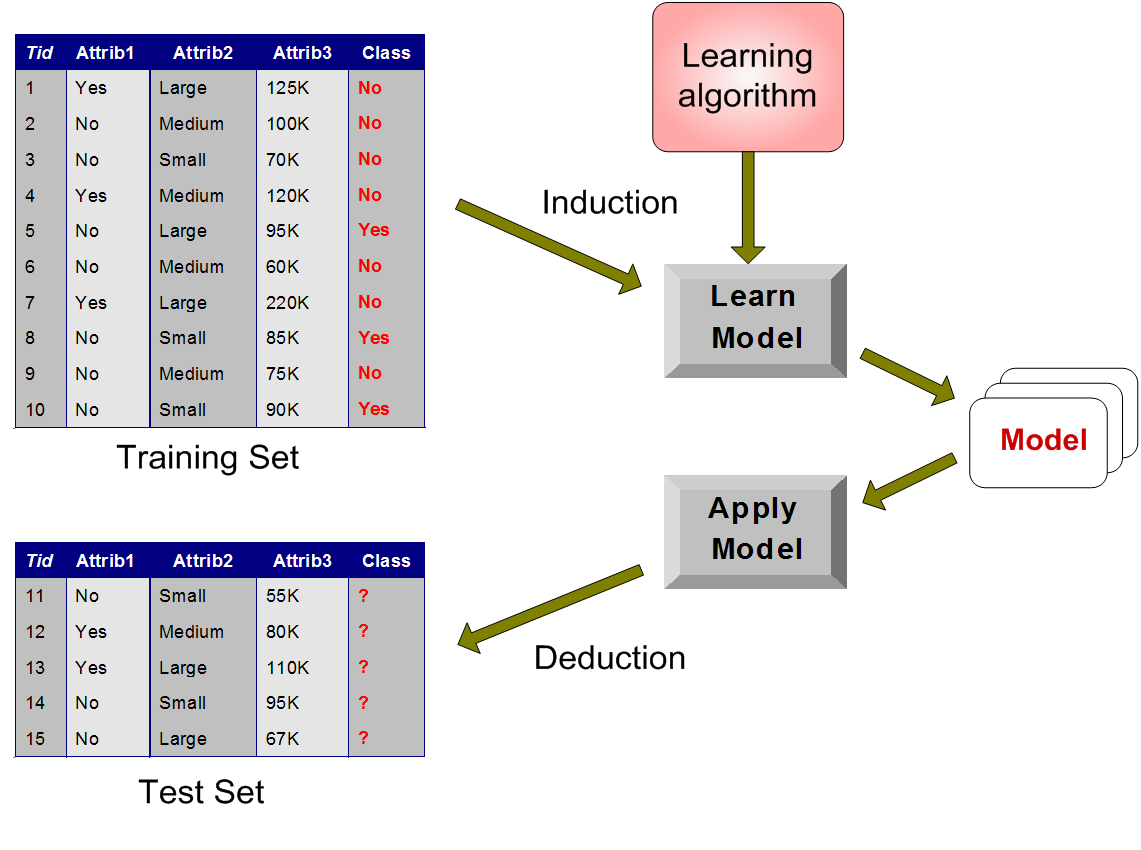
\includegraphics[width=0.8\linewidth,keepaspectratio]{traintest}
\end{center}

\tiny{(Reference: Data Mining Classification - Gun Ho Lee )}
\end{frame}


%%%%%%%%%%%%%%%%%%%%%%%%%%%%%%%%%%%%%%%%%%%%%%%%%%%%%%%%%%
\begin{frame}[fragile]\frametitle{Cross Validation: Measuring Performance}
\begin{itemize}
	\item Labeled training data is finite.
	\item The model built needs to be validated. 
	\item So, training data itself is split 
	\begin{itemize}
		\item Use one part for model building: Training Data.
		\item Use the other part: Testing Data. (actually called as Validation Data, but within Cross Validation process, it can be called as Testing data. Otherwise Testing data is the one which does not have output values. Validation data has output values for comparison.)
	\end{itemize}

\end{itemize}
\end{frame}

%%%%%%%%%%%%%%%%%%%%%%%%%%%%%%%%%%%%%%%%%%%%%%%%%%%%%%%%%%%
%\begin{frame}[fragile]\frametitle{Cross Validation}
%\begin{itemize}
%	\item Model predicts. Compare with known labels from Testing data
%	\item Error to be minimized.
%	\item Once error is min.
%	\item Unseen test data is fed for prediction
%\end{itemize}
%\end{frame}

%%%%%%%%%%%%%%%%%%%%%%%%%%%%%%%%%%%%%%%%%%%%%%%%%%%%%%%%%%
\begin{frame}[fragile]\frametitle{Machine Learning Technique}
\begin{center}
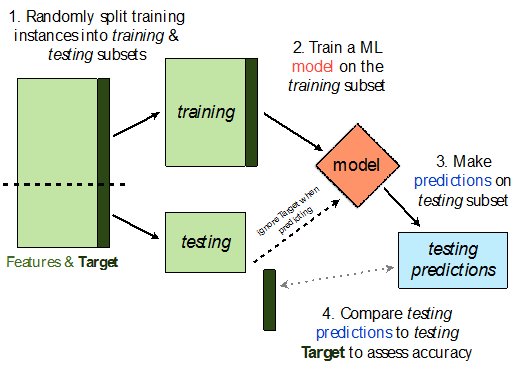
\includegraphics[width=0.75\linewidth,keepaspectratio]{crossval1}
\end{center}
%\tiny{(Reference: https://www.developer.com/mgmt/real-world-machine-learning-model-evaluation-and-optimization.html)}
\end{frame}



% %%%%%%%%%%%%%%%%%%%%%%%%%%%%%%%%%%%%%%%%%%%%%%%%%%%%%%%%%
% \begin{frame}[fragile]\frametitle{Cross Validation}
% % \begin{center}
% % 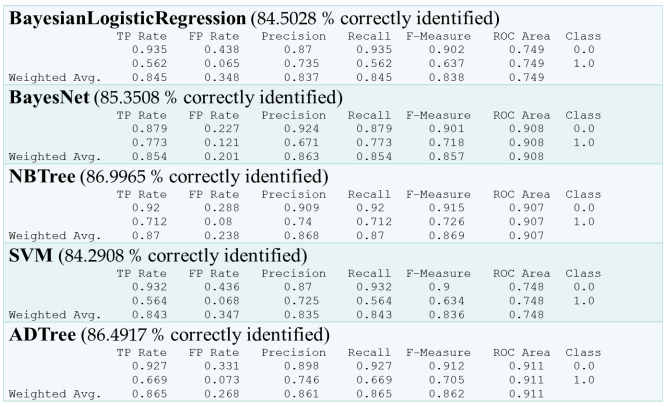
\includegraphics[width=0.6\linewidth,keepaspectratio]{crossval}
% % \end{center}
% \begin{center}
% 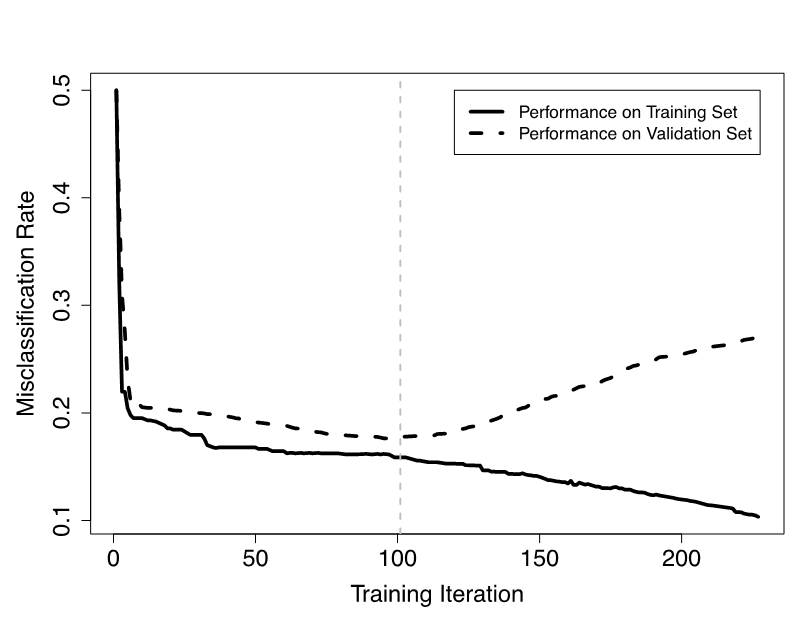
\includegraphics[width=0.6\linewidth,keepaspectratio]{crosstest}
% \end{center}
% \end{frame}

%%%%%%%%%%%%%%%%%%%%%%%%%%%%%%%%%%%%%%%%%%%%%%%%%%%%%%%%%%
\begin{frame}[fragile]\frametitle{Cross Validation}
How to divide dataset into Training, Validation, Testing sets?
\begin{itemize}
\item Problems?
	\begin{itemize}
	\item Validation set should ``represent'' the Training set.
	\item ``Lucky split'' is possible: Difficult instances were chosen for the training set, Easy instances put into the testing set
	\end{itemize}
\item Multiple evaluations using different portions of data for training and validating/testing
\item k-fold Cross Validation
\end{itemize}
\end{frame}

%%%%%%%%%%%%%%%%%%%%%%%%%%%%%%%%%%%%%%%%%%%%%%%%%%%%%%%%%%
\begin{frame}[fragile]\frametitle{K-Fold}
\begin{center}
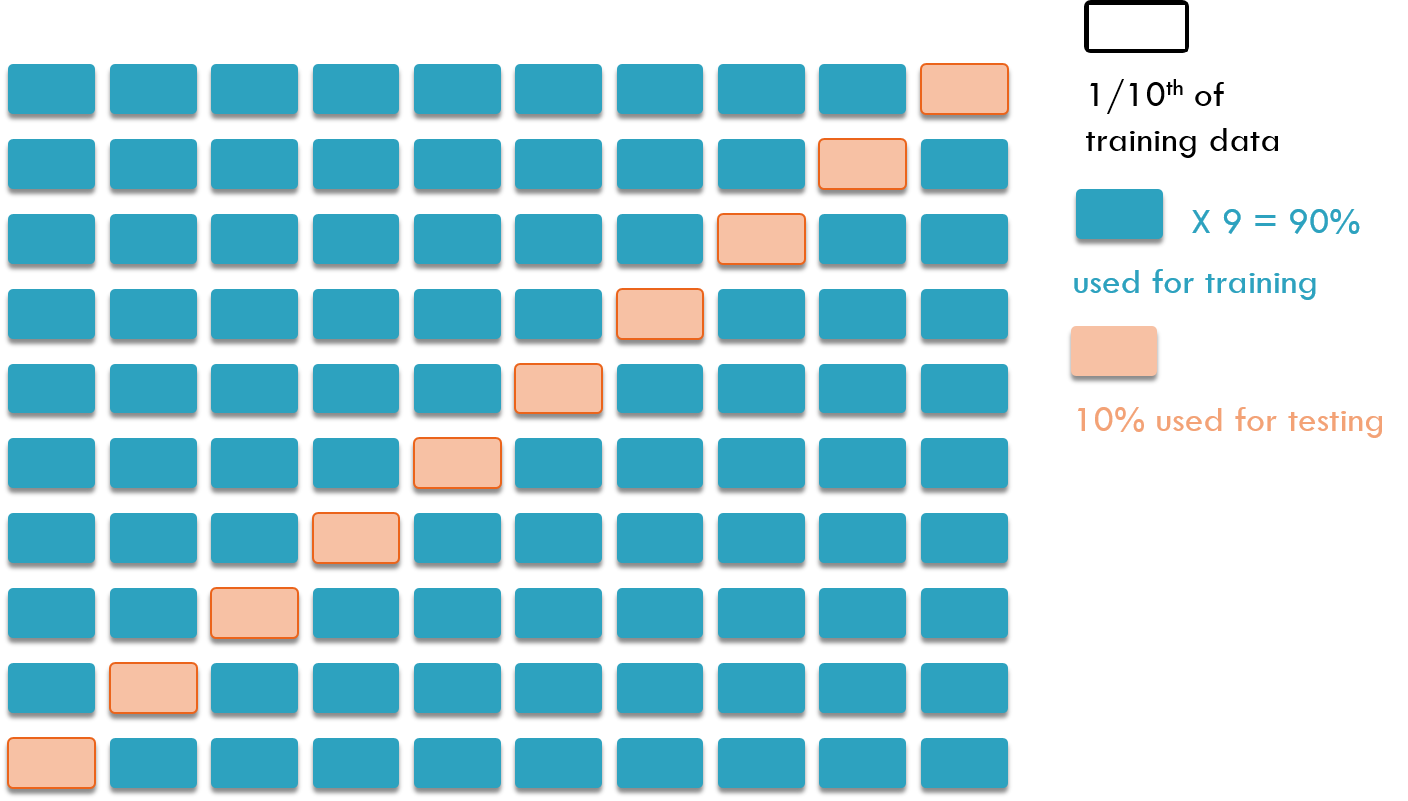
\includegraphics[width=0.75\linewidth,keepaspectratio]{kfold}
\end{center}

Cross Validation Error Estimate: $= \frac{1}{k} \sum Error_i$

Note: Here weights or all 10 models are neither averaged nor the last weights are taken as final model. [PTO]
\end{frame}




%%%%%%%%%%%%%%%%%%%%%%%%%%%%%%%%%%%%%%%%%%%%%%%%%%%%%%%%%%
\begin{frame}[fragile]\frametitle{Practical Tip}

		\begin{itemize}

			\item Cross Validation is NOT used for Model Building, but choosing best model amongst choices such as Linear models, decision tree, SVM, etc. 
			\item Once a specific model with known hyper parameters is finalized using least average error, a new model is built using FULL training data. 
			\item Not splits are done there.
					\end{itemize}
\end{frame}

% %%%%%%%%%%%%%%%%%%%%%%%%%%%%%%%%%%%%%%%%%%%%%%%%%%%%%%%%%%
% \begin{frame}[fragile]\frametitle{Machine Learning in Production}
% \begin{center}
% 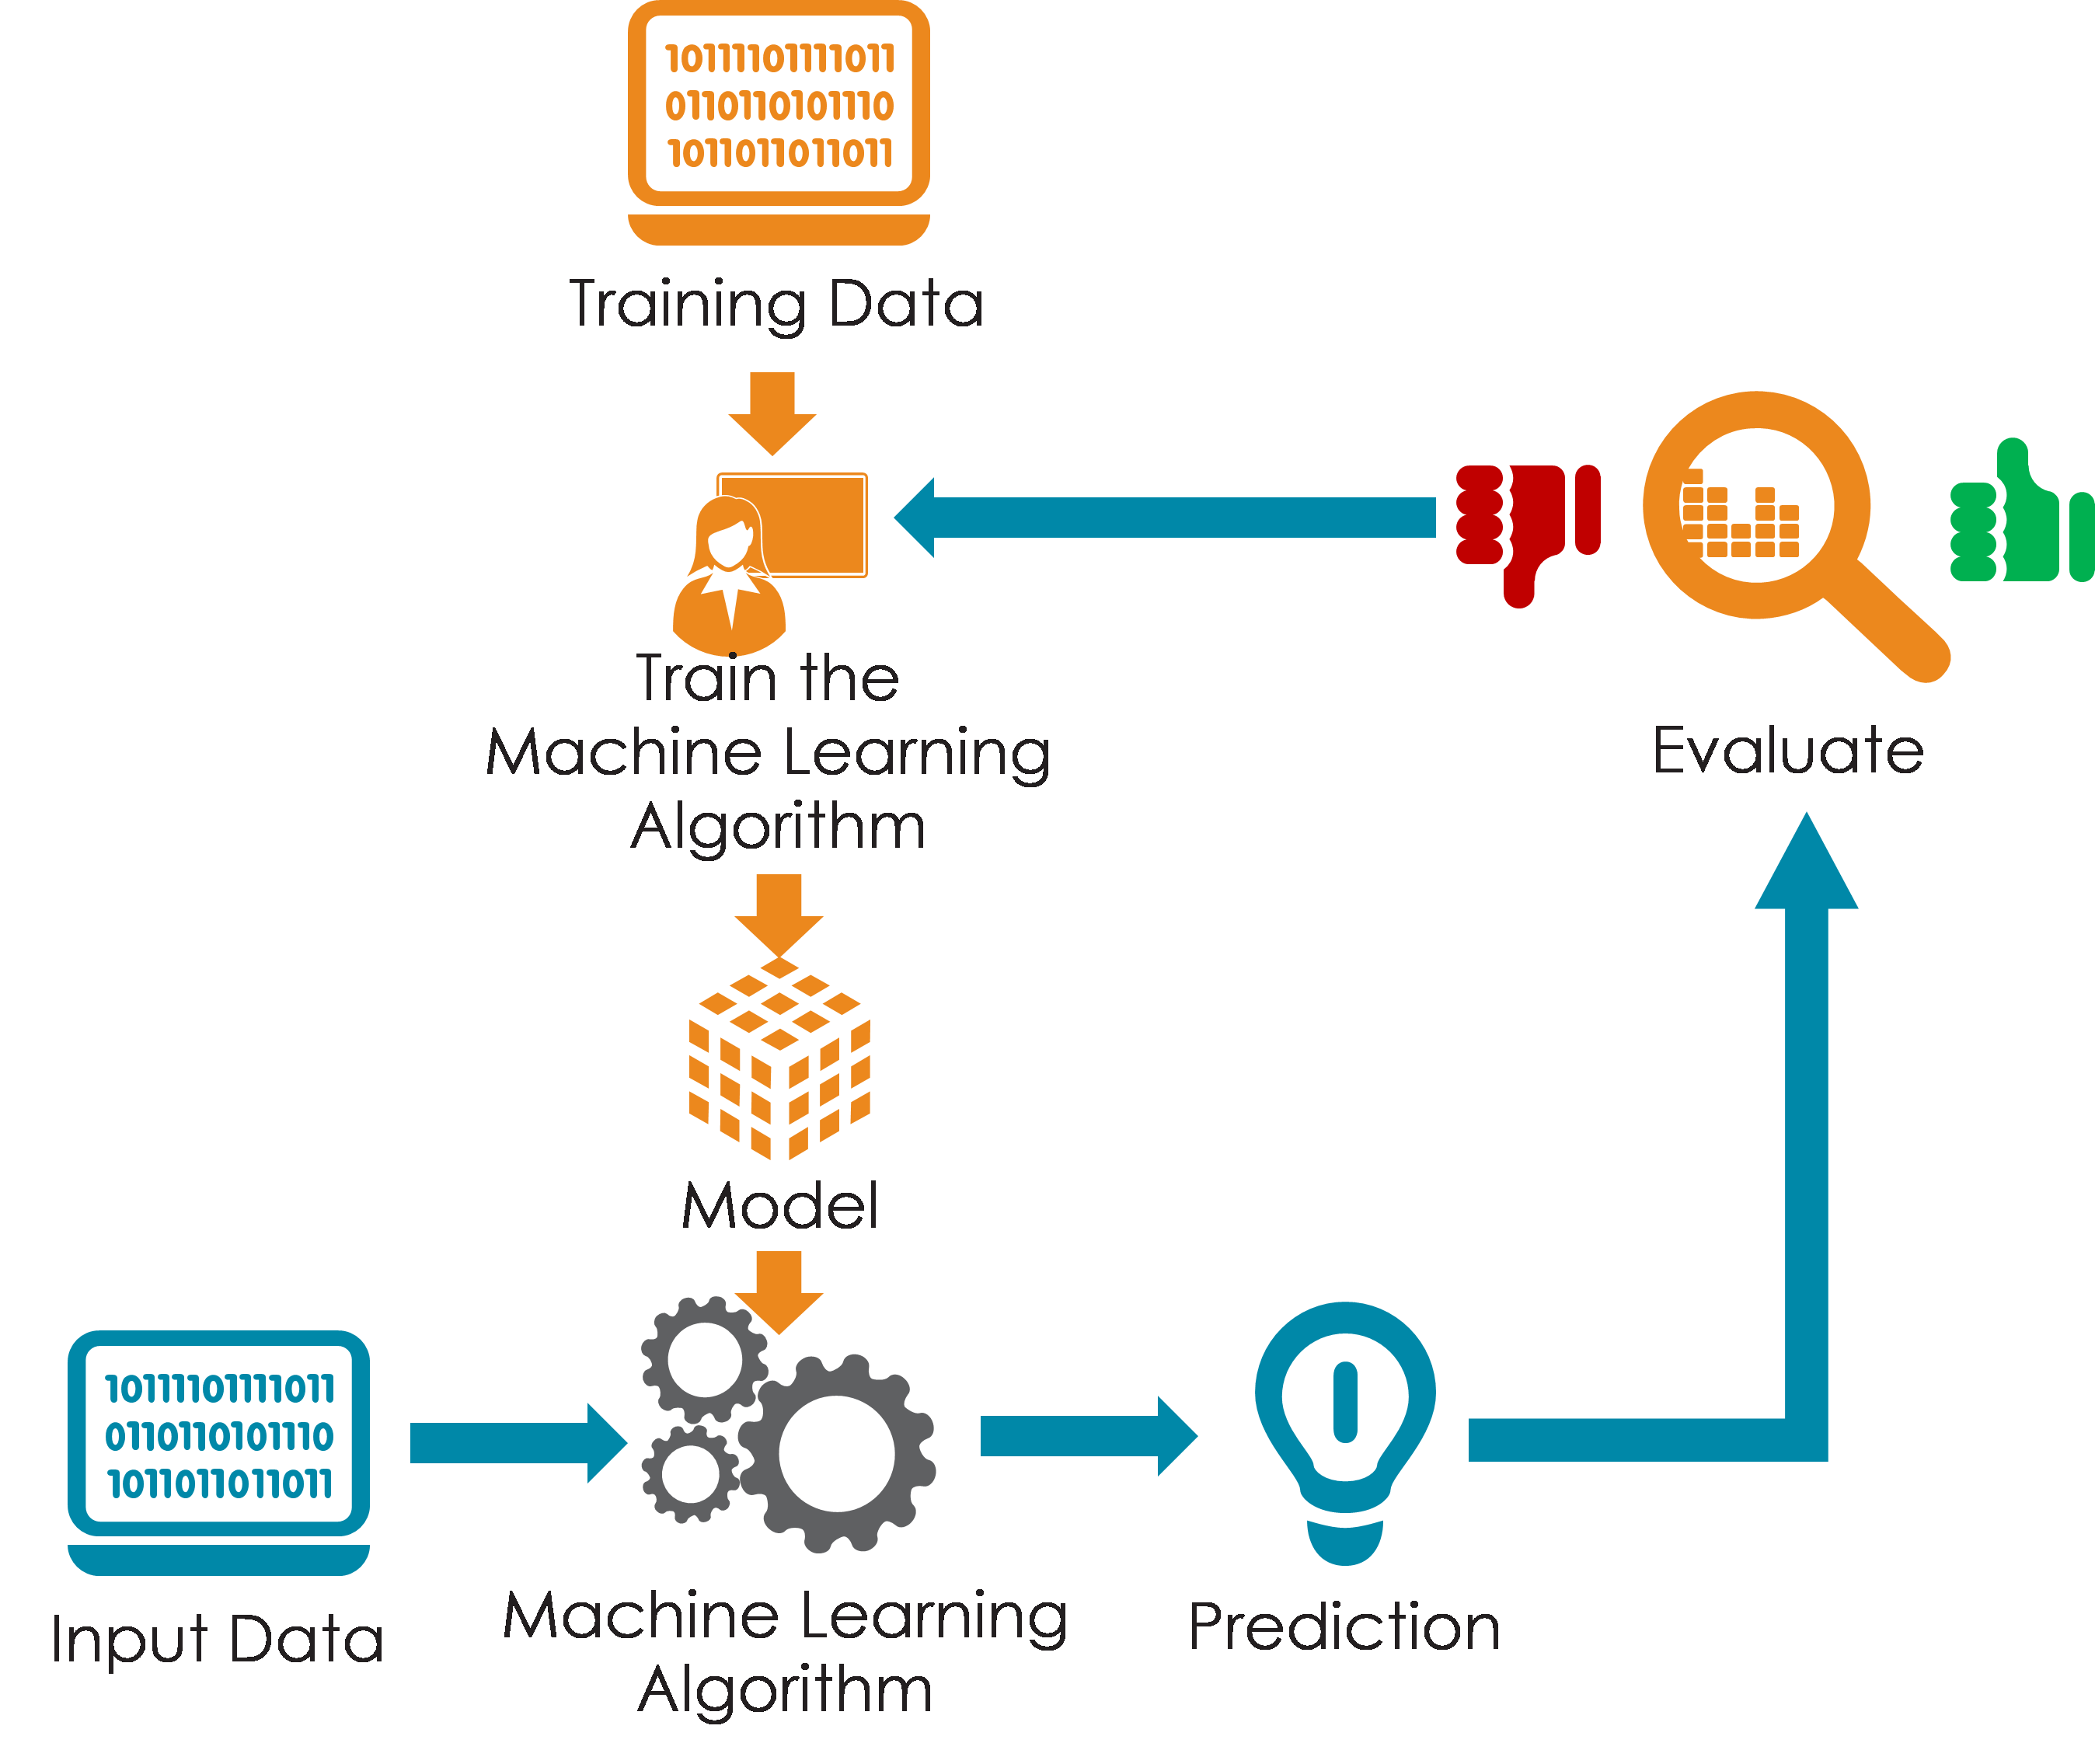
\includegraphics[width=0.7\linewidth,keepaspectratio]{mlteq1}
% \end{center}
% \tiny{(Reference: Building the Machine Learning Infrastructure - Data Points, Teradata)}
% \end{frame}

% %%%%%%%%%%%%%%%%%%%%%%%%%%%%%%%%%%%%%%%%%%%%%%%%%%%%%%%%%%%%%%%%%%%%%%%%%%%%%%%%%%
% \begin{frame}[fragile]\frametitle{}
% \begin{center}
% {\Large Machine Learning Algorithms}
% \end{center}
% \end{frame}


% %%%%%%%%%%%%%%%%%%%%%%%%%%%%%%%%%%%%%%%%%%%%%%%%%%%%%%%%%%
% \begin{frame}[fragile]\frametitle{Types of Machine Learning}
% \begin{itemize}
	% \item {\bf Supervised Learning}: Inputs and outputs are needed for training. Model finds the map and is used to predict the unseen.
	% \item {\bf Unsupervised Learning}: Outputs are not provided. Pattern/clusters finding.
	% \item {\bf Reinforcement Learning}:  The machine is exposed to an environment where it trains itself continually.
% \end{itemize}
% \end{frame}

%%%%%%%%%%%%%%%%%%%%%%%%%%%%%%%%%%%%%%%%%%%%%%%%%%%%%%%%%%%
%\begin{frame}[fragile]\frametitle{Supervised Learning}
%\begin{center}
%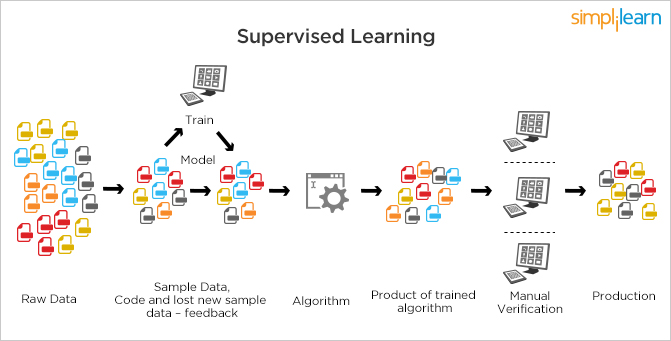
\includegraphics[width=\linewidth,keepaspectratio]{suplearn1}
%\end{center}
%\tiny{(Reference: Machine Learning: What it is and Why it Matters - Simplilearn)}
%\end{frame}
%
%%%%%%%%%%%%%%%%%%%%%%%%%%%%%%%%%%%%%%%%%%%%%%%%%%%%%%%%%%%
%\begin{frame}[fragile]\frametitle{Unsupervised Learning}
%\begin{center}
%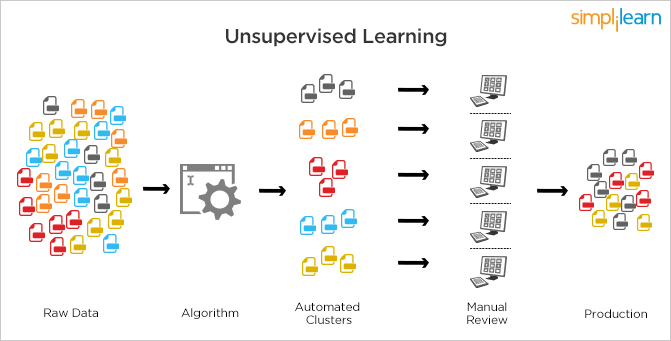
\includegraphics[width=\linewidth,keepaspectratio]{unsuplearn1}
%\end{center}
%\tiny{(Reference: Machine Learning: What it is and Why it Matters - Simplilearn)}
%\end{frame}
%
%
%%%%%%%%%%%%%%%%%%%%%%%%%%%%%%%%%%%%%%%%%%%%%%%%%%%%%%%%%%%
%\begin{frame}[fragile]\frametitle{Reinforcement Learning}
%\begin{center}
%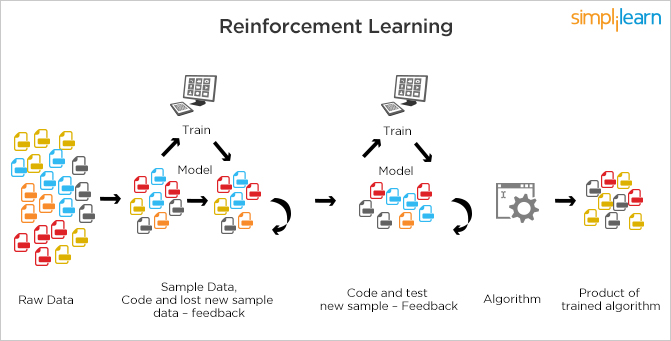
\includegraphics[width=\linewidth,keepaspectratio]{reinlearn}
%\end{center}
%\tiny{(Reference: Machine Learning: What it is and Why it Matters - Simplilearn)}
%\end{frame}

%%%%%%%%%%%%%%%%%%%%%%%%%%%%%%%%%%%%%%%%%%%%%%%%%%%%%%%%%%%%%%%%%%%%%%%%%%%%%%%%%%
\begin{frame}[fragile]\frametitle{}
\begin{center}
{\Large Machine Learning Evaluation}
\end{center}
\end{frame}

%%%%%%%%%%%%%%%%%%%%%%%%%%%%%%%%%%%%%%%%%%%%%%%%%%%%%%%%%
\begin{frame}[fragile]\frametitle{Evaluation}
Given Actuals and Predictions, how to find out how good the performance was?
\begin{itemize}
\item Accuracy: Misclassification Rate
\item Confusion Matrix
\item Precision, Recall, F1
\end{itemize}
%Experiments:
%\begin{itemize}
%\item Cross-Validation
%\item Bootstrap
%\item Out-of-time Sampling
%\end{itemize}
\end{frame}

%%%%%%%%%%%%%%%%%%%%%%%%%%%%%%%%%%%%%%%%%%%%%%%%%%%%%%%%%%%%%%%%%%%%%%%%%%%%%%%%%%
\begin{frame}[fragile]\frametitle{}
\begin{center}
{\Large Evaluation Metrics: Accuracy}
\end{center}
\end{frame}

%%%%%%%%%%%%%%%%%%%%%%%%%%%%%%%%%%%%%%%%%%%%%%%%%%%%%%%%%%
\begin{frame}[fragile]\frametitle{Accuracy}
Model Evaluation on Test Set (Regression) - Mean Squared Error
\begin{itemize}
\item Mean Squared Error: measuring the ``quality of fit''
\item Will be small if the predicted responses are very close to the true responses
$MSE = \frac{1}{n} \sum (y_i - f(x_i))^2$
\end{itemize}
\end{frame}

%%%%%%%%%%%%%%%%%%%%%%%%%%%%%%%%%%%%%%%%%%%%%%%%%%%%%%%%%
\begin{frame}[fragile]\frametitle{Accuracy}
How should classifier be quantitatively evaluated?
\begin{itemize}
\item Misclassification Rate = $\frac{NumIncorrectPrediction}{TotalPrediction}$
\item Issues with misclassification rate?
	\begin{itemize}
	\item If Accuracy is used: Example: in CC fraud domain, there are many more legitimate transactions than fraudulent transactions
	\item Then: Classifier that predicts every transaction as GOOD would have 99\% accuracy! Seems great, but it's not
	\end{itemize}
\end{itemize}

\end{frame}


%%%%%%%%%%%%%%%%%%%%%%%%%%%%%%%%%%%%%%%%%%%%%%%%%%%%%%%%%%%%%%%%%%%%%%%%%%%%%%%%%%
\begin{frame}[fragile]\frametitle{}
\begin{center}
{\Large Evaluation Metrics: Confusion Matrix}
\end{center}
\end{frame}


%%%%%%%%%%%%%%%%%%%%%%%%%%%%%%%%%%%%%%%%%%%%%%%%%%%%%%%%%
%\begin{frame}[fragile]\frametitle{Evaluation Metrics}
%How should classifier be quantitatively evaluated?
%\begin{equation}
%			Accuracy = \frac{Number Of Correct Predictions}{Total Number Of Predictions} =
%			\frac{f_{11} + f_{00}}{f_{11} + f_{10} + f_{01} + f_{00}}
%		\end{equation}
%		\begin{equation}
%			Error Rate = \frac{Number Of Wrong Predictions}{Total Number Of Predictions} =
%			\frac{f_{10} + f_{01}}{f_{11} + f_{10} + f_{01} + f_{00}}
%\end{equation}
%\end{frame}

%%%%%%%%%%%%%%%%%%%%%%%%%%%%%%%%%%%%%%%%%%%%%%%%%%%%%%%%%%
\begin{frame}[fragile]\frametitle{Evaluation Metrics}
There are predicted labels (Positive / negative) as well as actual labels (Positive / negative) .
\begin{center}
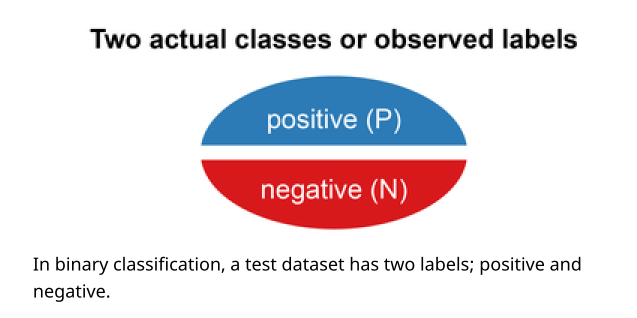
\includegraphics[width=0.8\linewidth,keepaspectratio]{confmat1}
\end{center}

% % (Ref: https://classeval.wordpress.com/introduction/basic-evaluation-measures/)
\end{frame}

%%%%%%%%%%%%%%%%%%%%%%%%%%%%%%%%%%%%%%%%%%%%%%%%%%%%%%%%%%
\begin{frame}[fragile]\frametitle{Evaluation Metrics}
The predicted labels will be exactly the same if the performance of a binary
classifier is perfect, but it is uncommon to be able to develop a perfect binary
classifier that is practical for various conditions.
\begin{center}
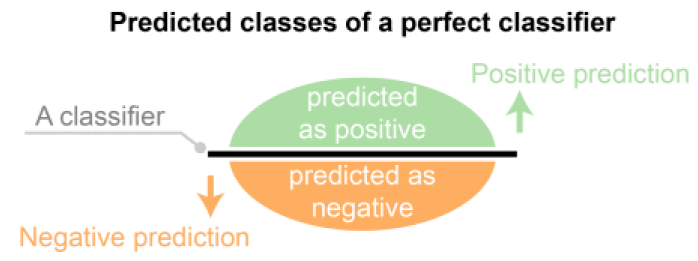
\includegraphics[width=0.8\linewidth,keepaspectratio]{confmat2}
\end{center}

\end{frame}

%%%%%%%%%%%%%%%%%%%%%%%%%%%%%%%%%%%%%%%%%%%%%%%%%%%%%%%%%%
\begin{frame}[fragile]\frametitle{Evaluation Metrics}
Hence, the predicted labels usually match with part of the observed labels
\begin{center}
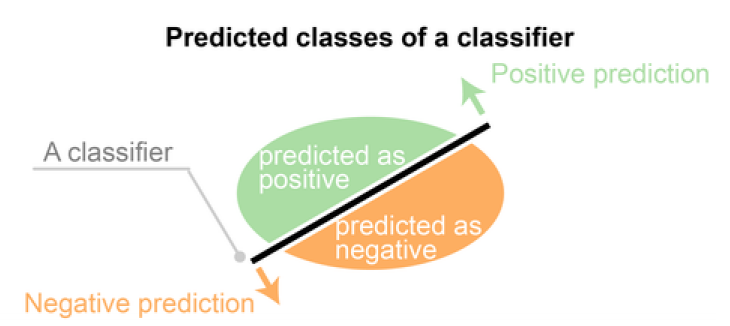
\includegraphics[width=0.8\linewidth,keepaspectratio]{confmat3}
\end{center}

\end{frame}
%
%%%%%%%%%%%%%%%%%%%%%%%%%%%%%%%%%%%%%%%%%%%%%%%%%%%%%%%%%%%
%\begin{frame}[fragile]\frametitle{Evaluation Metrics}
%A confusion matrix is formed from the four outcomes produced as a result of binary
%classification.
%	\begin{itemize}
%	\item True Positive (TP): number of positive examples correctly predicted by model
%	\item False Negative (FN): number of positive examples wrongly predicted as negative
%	\item False Positive (FP): number of negative examples wrongly predicted as positive
%	\item True Negative (TN): number of negative examples correctly predicted
%	\end{itemize}
%
%\end{frame}

%%%%%%%%%%%%%%%%%%%%%%%%%%%%%%%%%%%%%%%%%%%%%%%%%%%%%%%%%%
\begin{frame}[fragile]\frametitle{Evaluation Metrics}
Classification of a test dataset produces four outcomes - true positive, false positive,
true negative, and false negative.
\begin{center}
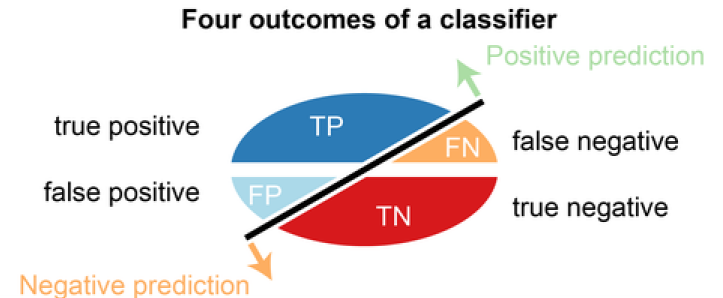
\includegraphics[width=0.8\linewidth,keepaspectratio]{confmat4}
\end{center}
Error rate (ERR) and accuracy (ACC) are the most common and intuitive measures
derived from the confusion matrix.
\end{frame}

%%%%%%%%%%%%%%%%%%%%%%%%%%%%%%%%%%%%%%%%%%%%%%%%%%%%%%%%%%
\begin{frame}[fragile]\frametitle{Error rate (ERR)}

\begin{center}
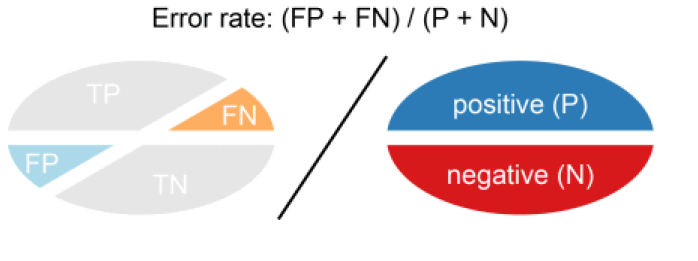
\includegraphics[width=0.8\linewidth,keepaspectratio]{confmat5}
\end{center}
It is calculated as the number of all incorrect predictions divided by
the total number of the dataset. The best error rate is 0.0, whereas the worst is 1.

$ERR = \frac{FP + FN}{TP+TN+FN+FP} = \frac{FP+FN}{P+N}$
\end{frame}

%%%%%%%%%%%%%%%%%%%%%%%%%%%%%%%%%%%%%%%%%%%%%%%%%%%%%%%%%%
\begin{frame}[fragile]\frametitle{Accuracy}

It is calculated as the number of all  correct predictions divided by the
total number of the dataset. The best accuracy is 1.0, whereas the worst is 0.0. It can
also be calculated by $1 - ERR$.

\begin{center}
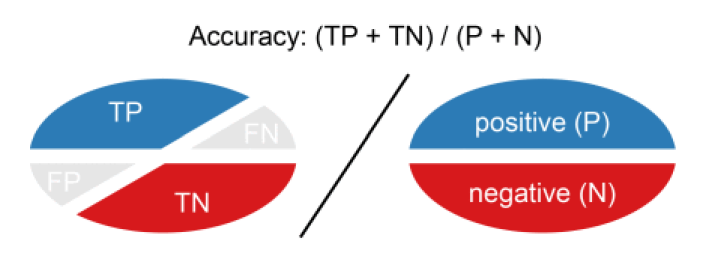
\includegraphics[width=0.8\linewidth,keepaspectratio]{confmat6}
\end{center}

$Accuracy = \frac{TP+TN}{P+N}$
\end{frame}


%%%%%%%%%%%%%%%%%%%%%%%%%%%%%%%%%%%%%%%%%%%%%%%%%%%%%%%%%%
\begin{frame}[fragile]\frametitle{Sensitivity (Recall or True positive rate)}

Sensitivity (SN) is calculated as the number of correct positive predictions divided by
the total number of positives. It is also called recall (REC) or true positive rate (TPR). The best sensitivity is 1.0, whereas the worst is 0.0.

\begin{center}
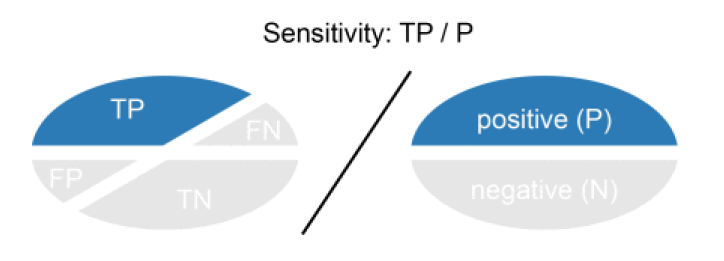
\includegraphics[width=0.8\linewidth,keepaspectratio]{confmat7}
\end{center}

$SN = \frac{TP}{TP+FN} = \frac{TP}{P}$
\end{frame}

%%%%%%%%%%%%%%%%%%%%%%%%%%%%%%%%%%%%%%%%%%%%%%%%%%%%%%%%%%
\begin{frame}[fragile]\frametitle{Specificity (True negative rate)}

Specificity (SP) is calculated as the number of correct negative predictions divided by
the total number of negatives. It is also called true negative rate (TNR). The best
specificity is 1.0, whereas the worst is 0.0.

\begin{center}
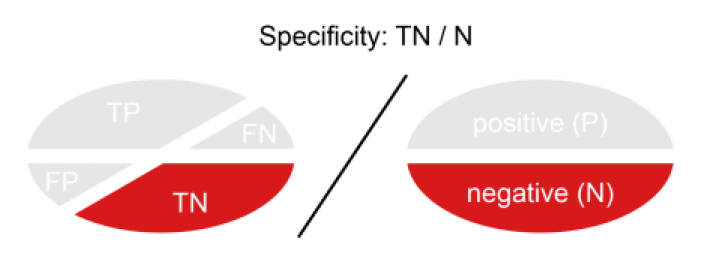
\includegraphics[width=0.8\linewidth,keepaspectratio]{confmat8}
\end{center}

$SP = \frac{TN}{TN+FP} = \frac{TN}{N}$
\end{frame}


%%%%%%%%%%%%%%%%%%%%%%%%%%%%%%%%%%%%%%%%%%%%%%%%%%%%%%%%%%
\begin{frame}[fragile]\frametitle{Sensitivity vs Specificity}

	\begin{itemize}
	\item For sensitivity we will look oat only *P, all that were predicted positive, rest are all in the negatives group.
	\item For highly sensitive test, 100\% sensitive, within the Negatives group, there is no mistake. 
	\item Meaning anyone who has tested negative, they surely don't have disease.
	\item All are truly negative. Meaning FN are 0. Recall thus can be made 1 by marking all positive. So there is no one in the Negatives group. So no FN. But thats not good.
	\item But still its not a perfect test, because within Positives, you may have some FPs.
	\item Similarly 100\% Specific test: We will send all negative tested guys to a different group. Within them we had FN guys as well. The Positives were perfect. All of them had disease. $FP=0$. So those who tested positive surely had the disease.
	\item In reality there is no perfect test!!
	\end{itemize}

\end{frame}


%%%%%%%%%%%%%%%%%%%%%%%%%%%%%%%%%%%%%%%%%%%%%%%%%%%%%%%%%%
\begin{frame}[fragile]\frametitle{Precision (Positive predictive value)}
Precision (PREC) is calculated as the number of correct positive predictions divided
by the total number of positive predictions. It is also called positive predictive value
(PPV). The best precision is 1.0, whereas the worst is 0.0.

\begin{center}
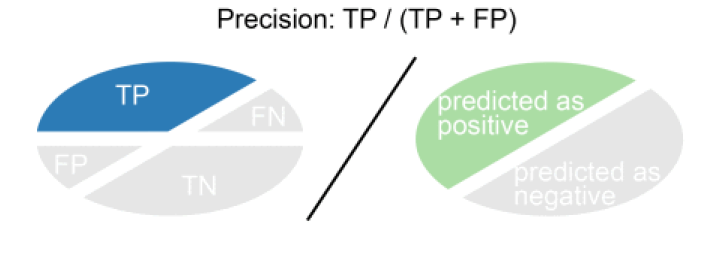
\includegraphics[width=0.8\linewidth,keepaspectratio]{confmat9}
\end{center}

$PREC = \frac{TP}{TP+FP}$
\end{frame}

%%%%%%%%%%%%%%%%%%%%%%%%%%%%%%%%%%%%%%%%%%%%%%%%%%%%%%%%%%
\begin{frame}[fragile]\frametitle{False positive rate}
False positive rate (FPR) is calculated as the number of incorrect positive predictions
divided by the total number of negatives. The best false positive rate is 0.0 whereas
the worst is 1.0. It can also be calculated as 1 - specificity.

\begin{center}
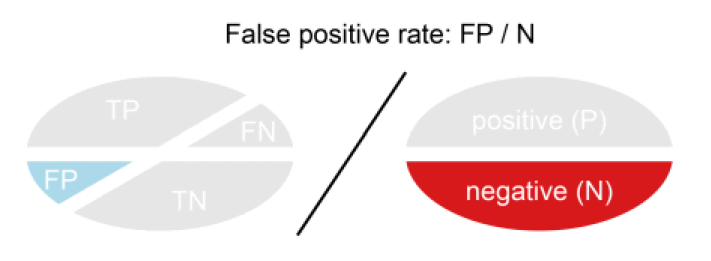
\includegraphics[width=0.8\linewidth,keepaspectratio]{confmat10}
\end{center}

$FPR  = \frac{FP}{TN+FP} = 1 - SP$
\end{frame}




%%%%%%%%%%%%%%%%%%%%%%%%%%%%%%%%%%%%%%%%%%%%%%%%%%%%%%%%%%
\begin{frame}[fragile]\frametitle{Example}
\begin{center}
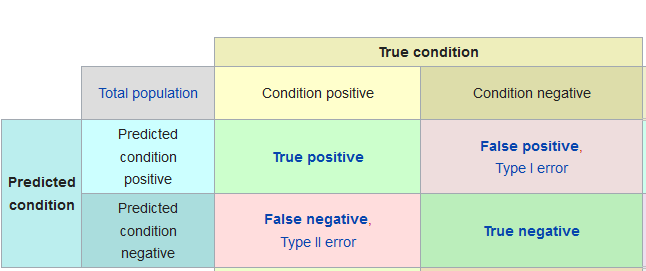
\includegraphics[width=0.9\linewidth,keepaspectratio]{confmat}
\end{center}
\end{frame}

%%%%%%%%%%%%%%%%%%%%%%%%%%%%%%%%%%%%%%%%%%%%%%%%%%%%%%%%%%
\begin{frame}[fragile]\frametitle{Type I Error}
Type I Error is equivalent to False Positive (FP).
	\begin{itemize}
	\item Test is Positive but actually diesese is not there.
	\item A Fire alarm going off when in fact there is no fire. 
	\end{itemize}
This kind of error is synonymous to ``believing a lie'' or ``a false alarm''.
\end{frame}

%%%%%%%%%%%%%%%%%%%%%%%%%%%%%%%%%%%%%%%%%%%%%%%%%%%%%%%%%%
\begin{frame}[fragile]\frametitle{Type II Error}
Type II Error is equivalent to False Negative (FN). 

	\begin{itemize}
	\item Test is Negative but actually diesese is there..
	\item A Fire breaking out and the fire alarm does not ring. 
	\end{itemize}
This kind of error is synonymous to ``failing to believe a truth'' or ``a miss''.
\end{frame}

%%%%%%%%%%%%%%%%%%%%%%%%%%%%%%%%%%%%%%%%%%%%%%%%%%%%%%%%%%
\begin{frame}[fragile]\frametitle{Errors}
\begin{center}
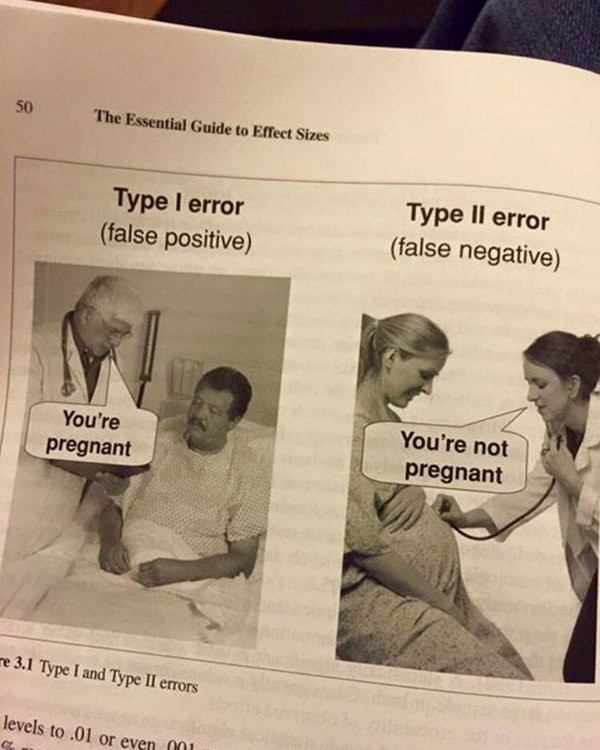
\includegraphics[width=0.5\linewidth,keepaspectratio]{confmat11}
\end{center}
\end{frame}




%%
%%
%%%%%%%%%%%%%%%%%%%%%%%%%%%%%%%%%%%%%%%%%%%%%%%%%%%%%%%%%%%%
%%\begin{frame}[fragile]\frametitle{Confusion Matrix: Percentages}
%%\begin{itemize}
%%\item True Positive Rate (TPR): fraction of positive examples correctly predicted by model. Sensitivity $=\frac{TP}{(TP+FN)}$
%%\item False Negative Rate (FNR): fraction of positive examples wrongly predicted as negative $=\frac{FN}{(TP+FN)}$
%%\item False Positive Rate (FPR): fraction of negative examples wrongly predicted as positive $=\frac{FP}{(TN+FP)}$
%%\item True Negative Rate (TNR): fraction of negative examples correctly predicted. Also referred to as specificity $=\frac{TN}{(TN+FP)}$
%%\end{itemize}
%%\begin{center}
%%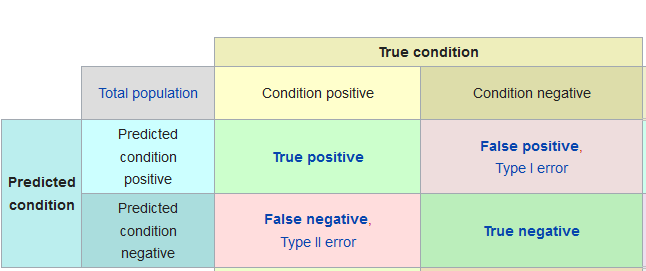
\includegraphics[width=0.8\linewidth,keepaspectratio]{confmat}
%%\end{center}
%%
%%\end{frame}

%%%%%%%%%%%%%%%%%%%%%%%%%%%%%%%%%%%%%%%%%%%%%%%%%%%%%%%%%%%%
%%\begin{frame}[fragile]\frametitle{Confusion Matrix: Classification}
%%		\begin{table}[h]
%%		\centering
%%			\begin{tabular}{| l | l | l | l |}
%%				\hline
%%				\multicolumn{2}{| l |}{\multirow{2}{*}{ }} & \multicolumn{2}{| l |}{Predicted class} \\ \cline{3-4} 
%%				 & & Class = 1 & Class = 0 \\ \hline
%%				\multirow{2}{*}{Actual class} & Class = 1 & $f_{11}$ & $f_{10}$ \\ \cline{2-4}
%%					& Class = 0 & $f_{01}$ & $f_{00}$ \\ \hline
%%
%%			\end{tabular}
%%			\caption{Confusion matrix for a 2-class problem.}
%%\end{table}
%%\end{frame}

%%%%%%%%%%%%%%%%%%%%%%%%%%%%%%%%%%%%%%%%%%%%%%%%%%%%%%%%%%%%%%%%%%%%%%%%%%%%%%%%%%
\begin{frame}[fragile]\frametitle{}
\begin{center}
{\Large Evaluation Metrics: Precision and Recall}
\end{center}
\end{frame}

%%%%%%%%%%%%%%%%%%%%%%%%%%%%%%%%%%%%%%%%%%%%%%%%%%%%%%%%%%
\begin{frame}[fragile]\frametitle{Precision and Recall}
\begin{itemize}
\item Precision: fraction of records that are positive in the set of records that classifier predicted as positive
\item Interpretation: If the prediction is very stringent then getting all of them correct is likely, so more precise. Less (no) mis-predictions (FP) happens.
 \item Recall: fraction of positive records that are correctly predicted by classifier, out of all actual.
\item Interpretation: Criteria is relaxed so that maximum catch is  made. Less (no) mis-classification (FN) happens.
\end{itemize}
\end{frame}



%%%%%%%%%%%%%%%%%%%%%%%%%%%%%%%%%%%%%%%%%%%%%%%%%%%%%%%%%%
\begin{frame}[fragile]\frametitle{Precision and Recall}
\begin{center}
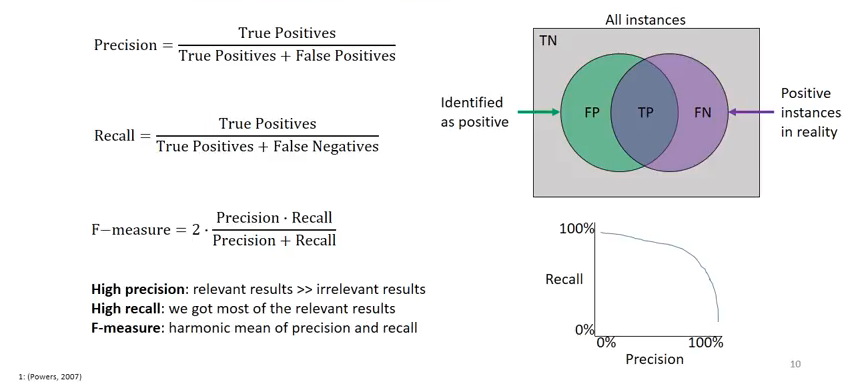
\includegraphics[width=\linewidth,keepaspectratio]{precisionrecall}
\end{center}
\tiny{(Reference: Text Mining - Jeff Shaul)}

\end{frame}


%%%%%%%%%%%%%%%%%%%%%%%%%%%%%%%%%%%%%%%%%%%%%%%%%%%%%%%%%%
\begin{frame}[fragile]\frametitle{F1 Measure}
\begin{itemize}
\item F-measure: combines precision and recall into a single metric, using the harmonic mean
\item Harmonic Mean of two numbers tends to be closer to the smaller of two numbers, so the only way F1 is high is for both precision and recall to be high.
 $F_1=\frac{2rp}{(r+p)}=\frac{2 \times TP}{(2 \times TP + FP + FN)}$
\end{itemize}

\begin{center}
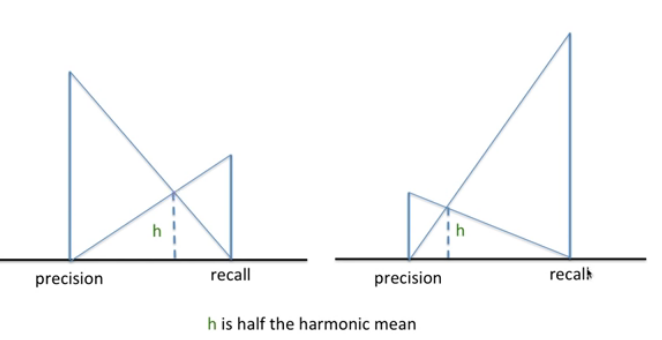
\includegraphics[width=0.6\linewidth,keepaspectratio]{f11}
\end{center}

Even if anyone is very high, we get balanced F1 score

\tiny{(Ref: Performance measure on multiclass classification - Minsuk Heo)}


\end{frame}

%%%%%%%%%%%%%%%%%%%%%%%%%%%%%%%%%%%%%%%%%%%%%%%%%%%%%%%%%%
\begin{frame}[fragile]\frametitle{F1 Measure}
\begin{itemize}
\item Model 1's F1 is better but Accuracy is lower than Model 2. Which is better?
\item F1 is better as it takes care of any imbalance in the targets.
\end{itemize}

\begin{center}
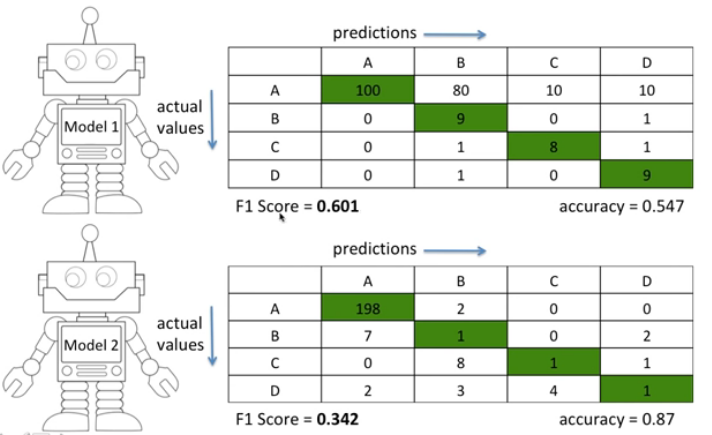
\includegraphics[width=0.6\linewidth,keepaspectratio]{f12}
\end{center}

\tiny{(Ref: Performance measure on multiclass classification - Minsuk Heo)}


\end{frame}

% %%%%%%%%%%%%%%%%%%%%%%%%%%%%%%%%%%%%%%%%%%%%%%%%%%%%%%%%%%
% \begin{frame}[fragile]\frametitle{Precision and Recall}
% \begin{itemize}
% \item Precision addresses False Positives and Recall addresses False Negatives
% \item So, if you are hunting something rare (skewed) like Cancer detection, Fraud, you are typically concerned with FN, as the test should not wrongly say that you have cancer. Use Recall.
% \item When you need to be very accurate then use Precision.
% \end{itemize}
% \end{frame}


% %%%%%%%%%%%%%%%%%%%%%%%%%%%%%%%%%%%%%%%%%%%%%%%%%%%%%%%%%%
% \begin{frame}[fragile]\frametitle{Precision and Recall}
% \begin{itemize}
% \item  Multi-class classification, the confusion matrix becomes n dimensional. 
% \item  Say, for 3 classes (labels)
% \item  Y axis is Predictions and X axis is for True values.
% \item Diagonals is where prediction of a class and the actual outcomes match (TPs)
% \item At other places, prediction was of some class and actual was something else.
% \item Precision calculations are per class basis and then average-ed.
% \end{itemize}

% \tiny{(Ref: mlcourse.ai. Lecture 5. Part 2. Classification metrics. Theory - Yury Kashnitsky)}

% \end{frame}


%%%%%%%%%%%%%%%%%%%%%%%%%%%%%%%%%%%%%%%%%%%%%%%%%%%%%%%%%%%%%%%%%%%%%%%%%%%%%%%%%%
\begin{frame}[fragile]\frametitle{}
\begin{center}
{\Large Precision and Recall: Tug of War}
\end{center}
\end{frame}


% %%%%%%%%%%%%%%%%%%%%%%%%%%%%%%%%%%%%%%%%%%%%%%%%%%%%%%%%%%%%%%%%%%%%%%%%
% \begin{frame}[fragile]\frametitle{An Aesop's Fable: The Boy Who Cried Wolf (compressed)}

% \begin{itemize}
% \item A shepherd boy gets bored tending the town's flock. To have some fun, he cries out, ''Wolf!'' even though no wolf is in sight. The villagers run to protect the flock, but then get really mad when they realize the boy was playing a joke on them.

% \item One night, the shepherd boy sees a real wolf approaching the flock and calls out, ''Wolf!'' The villagers refuse to be fooled again and stay in their houses. The hungry wolf turns the flock into lamb chops. The town goes hungry. Panic ensues.

% \item Let's make the following definitions:
	% \begin{itemize}
% \item ``Wolf'' is a positive class.
% \item ``No wolf'' is a negative class.
% \end{itemize}
% \end{itemize}
% % (Ref: https://developers.google.com/machine-learning/crash-course/classification/true-false-positive-negative)
% \end{frame}

% %%%%%%%%%%%%%%%%%%%%%%%%%%%%%%%%%%%%%%%%%%%%%%%%%%%%%%%%%%%%%%%%%%%%%%%%
% \begin{frame}[fragile]\frametitle{Evaluation Metrics: Precision, Recall}
% \begin{itemize}
% \item Precision: (True Positives) / (All Positive Predictions)
% \begin{itemize}
% \item When model said ''positive'' class, was it right?
% \item How precisely did it say ``Wolf'''?
% \item Intuition: Did the model cry ''wolf'' too often?
	% \end{itemize}
% \item Recall: (True Positives) / (All Actual Positives)
% \begin{itemize}
% \item Out of all the possible positives, how many did the model correctly identify?
% \item Of all the wolves that came to village, how many did we get?
% \item Intuition: Did it miss any wolves?
	% \end{itemize}
		% \end{itemize}

% % (Ref: https://developers.google.com/machine-learning/crash-course/classification/video-lecture)
% \end{frame}




% %%%%%%%%%%%%%%%%%%%%%%%%%%%%%%%%%%%%%%%%%%%%%%%%%%%%%%%%%%%%%%%%%%%%%%%%
% \begin{frame}[fragile]\frametitle{Evaluation Metrics: Precision, Recall}
% \begin{center}
% 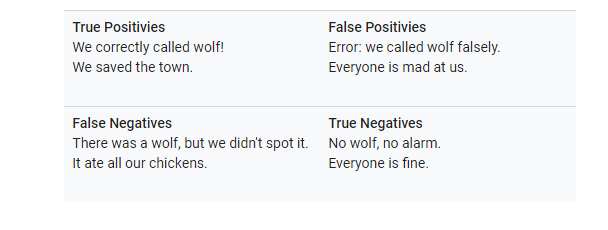
\includegraphics[width=0.8\linewidth]{logistic3}
% \end{center}


% % (Ref: https://developers.google.com/machine-learning/crash-course/classification/video-lecture)
% \end{frame}



% %%%%%%%%%%%%%%%%%%%%%%%%%%%%%%%%%%%%%%%%%%%%%%%%%%%%%%%%%%%%%%%%%%%%%%%%
% \begin{frame}[fragile]\frametitle{Evaluation Metrics: Recall}
% \begin{itemize}
% \item If you want to do better job at recall,  you need to be say ``Wolf'' more often. 
% \item Even when we just here some noise in the bushes. 
% \item We may be wrong at times. But thats fine. We don't want to miss any one. Collect more and more.
% \item Good recall comes when we lower the classification threshold. So we get more on positve side.
		% \end{itemize}

% % (Ref: https://developers.google.com/machine-learning/crash-course/classification/video-lecture)
% \end{frame}


% %%%%%%%%%%%%%%%%%%%%%%%%%%%%%%%%%%%%%%%%%%%%%%%%%%%%%%%%%%%%%%%%%%%%%%%%
% \begin{frame}[fragile]\frametitle{Evaluation Metrics: Precision}
% \begin{itemize}
% \item If you want to do better job at precision,  you need to be say ``Wolf'' only when you are absolutely sure, because you just don't want to be wrong. 
% \item Good precision comes when we higher the classification threshold. So we get less on positive side, but whatever small outcomes we get we are reasonably sure of them.
		% \end{itemize}

% % (Ref: https://developers.google.com/machine-learning/crash-course/classification/video-lecture)
% \end{frame}


%%%%%%%%%%%%%%%%%%%%%%%%%%%%%%%%%%%%%%%%%%%%%%%%%%%%%%%%%%%%%%%%%%%%%%%%
\begin{frame}[fragile]\frametitle{Precision and Recall: A Tug of War}
\begin{itemize}
\item Recall and Precision seem to be opposing each other.
\item Just knowing one value is not enough, but both
\item And we need to do better at both.

\end{itemize}

% (Ref: https://developers.google.com/machine-learning/crash-course/classification/video-lecture)
\end{frame}

%%%%%%%%%%%%%%%%%%%%%%%%%%%%%%%%%%%%%%%%%%%%%%%%%%%%%%%%%%%%%%%%%%%%%%%%
\begin{frame}[fragile]\frametitle{Precision and Recall: A Tug of War}
\begin{itemize}
\item Explore this notion by looking at the following figure, which shows 30 predictions made by an email classification model. 
\item Those to the right of the classification threshold are classified as "Spam", while those to the left are classified as "not Spam."
\end{itemize}

\begin{center}
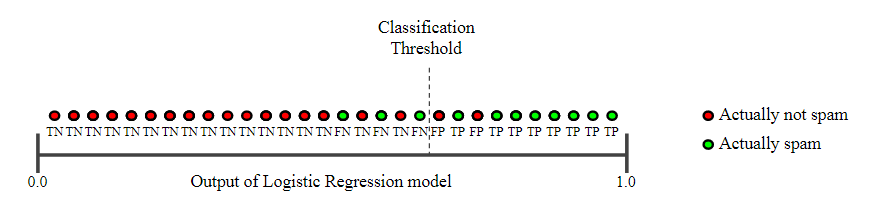
\includegraphics[width=\linewidth]{logistic6}
\end{center}

% (Ref: https://developers.google.com/machine-learning/crash-course/classification/video-lecture)
\end{frame}


%%%%%%%%%%%%%%%%%%%%%%%%%%%%%%%%%%%%%%%%%%%%%%%%%%%%%%%%%%
\begin{frame}[fragile]\frametitle{Precision and Recall trade-off}
\begin{itemize}
\item Typically to increase precision for a given model implies lowering recall, though this depends on the precision-recall curve of your model.
\item Generally, if you want higher precision you need to restrict the positive predictions to those with highest certainty in your model, which means predicting fewer positives overall (which, in turn, usually results in lower recall).
\item If you want to maintain the same level of recall while improving precision, you will need a better classifier.
\end{itemize}
\end{frame}


% %%%%%%%%%%%%%%%%%%%%%%%%%%%%%%%%%%%%%%%%%%%%%%%%%%%%%%%%%%%%%%%%%%%%%%%%
% \begin{frame}[fragile]\frametitle{Precision and Recall: A Tug of War}
% Let's calculate precision and recall based on the results 
% \begin{itemize}
% \item True Positives (TP): 8
% \item False Positives (FP): 2
% \item False Negatives (FN): 3
% \item True Negatives (TN): 17
% \end{itemize}


% % (Ref: https://developers.google.com/machine-learning/crash-course/classification/video-lecture)
% \end{frame}

% %%%%%%%%%%%%%%%%%%%%%%%%%%%%%%%%%%%%%%%%%%%%%%%%%%%%%%%%%%%%%%%%%%%%%%%%
% \begin{frame}[fragile]\frametitle{Precision and Recall: A Tug of War}
% Precision measures the percentage of emails flagged as Spam that were correctly classified-that is, the percentage of dots to the right of the threshold line that are green 

% $\text{Precision} = \frac{TP}{TP + FP} = \frac{8}{8+2} = 0.8$

% Recall measures the percentage of actual Spam emails that were correctly classified-that is, the percentage of green dots that are to the right of the threshold line

% $\text{Recall} = \frac{TP}{TP + FN} = \frac{8}{8 + 3} = 0.73$

% % (Ref: https://developers.google.com/machine-learning/crash-course/classification/video-lecture)
% \end{frame}

% %%%%%%%%%%%%%%%%%%%%%%%%%%%%%%%%%%%%%%%%%%%%%%%%%%%%%%%%%%%%%%%%%%%%%%%%
% \begin{frame}[fragile]\frametitle{Precision and Recall: A Tug of War}
% Now, this figure illustrates the effect of decreasing the classification threshold 
% \begin{center}
% 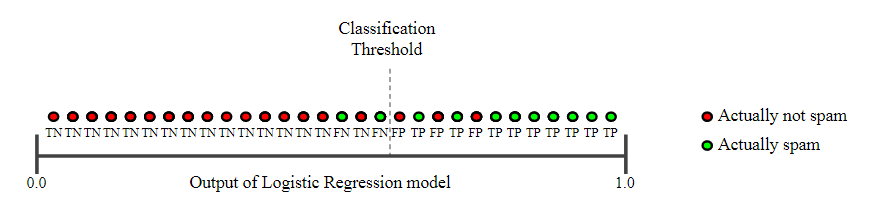
\includegraphics[width=\linewidth]{logistic7}
% \end{center}

% % (Ref: https://developers.google.com/machine-learning/crash-course/classification/video-lecture)
% \end{frame}

% %%%%%%%%%%%%%%%%%%%%%%%%%%%%%%%%%%%%%%%%%%%%%%%%%%%%%%%%%%%%%%%%%%%%%%%%
% \begin{frame}[fragile]\frametitle{Precision and Recall: A Tug of War}
% False positives increase, and false negatives decrease. As a result, this time, precision decreases and recall increases:

% \begin{itemize}
% \item True Positives (TP): 9
% \item False Positives (FP): 3
% \item False Negatives (FN): 2
% \item True Negatives (TN): 16
% \end{itemize}

% $\text{Precision} = \frac{TP}{TP + FP} = \frac{9}{9+3} = 0.75$

% $\text{Recall} = \frac{TP}{TP + FN} = \frac{9}{9 + 2} = 0.82$

% Various metrics have been developed that rely on both precision and recall, like F1.


% % (Ref: https://developers.google.com/machine-learning/crash-course/classification/video-lecture)
% \end{frame}

% %%%%%%%%%%%%%%%%%%%%%%%%%%%%%%%%%%%%%%%%%%%%%%%%%%%%%%%%%%%%%%%%%%%%%%%%
% \begin{frame}[fragile]\frametitle{Evaluation Metrics: Precision vs Recall}
% \begin{itemize}

% \item So which threshold is good, optimum?
% \item Try various thresholds and see, which one looks better.
% \end{itemize}

% % (Ref: https://developers.google.com/machine-learning/crash-course/classification/video-lecture)
% \end{frame}


%%%%%%%%%%%%%%%%%%%%%%%%%%%%%%%%%%%%%%%%%%%%%%%%%%%%%%%%%%
\begin{frame}[fragile]\frametitle{Precision and Recall trade-off : Summary}
\begin{itemize}
\item Intuitively, if you cast a wider net (meaning your classifier threshold is relaxed), you will detect more relevant documents/positive cases (higher recall) 
\item But you will also get more false alarms (lower precision). 
\item If you classify everything in the positive category, you have 100\% recall (no FN here), a bad precision because some of them could be wrong, so there will be many FPs, making precision lower.
\item If you adjust threshold strict so as to have good precision, you will have lower making of positives and mark many actually positive values as negative, falsely. Making more FNs, thus lower recall.
\end{itemize}
\end{frame}



%%%%%%%%%%%%%%%%%%%%%%%%%%%%%%%%%%%%%%%%%%%%%%%%%%%%%%%%%%%%%%%%%%%%%%%%%%%%%%%%%%
\begin{frame}[fragile]\frametitle{}
\begin{center}
{\Large Machine Learning Model Generalization}
\end{center}
\end{frame}


%%%%%%%%%%%%%%%%%%%%%%%%%%%%%%%%%%%%%%%%%%%%%%%%%%%%%%%%%%
\begin{frame}[fragile]\frametitle{Generalization in Machine Learning}
\begin{itemize}
\item Generalization refers to how well the concepts learned by a machine learning model apply to specific examples not seen by the model when it was learning.
\item The goal of a good machine learning model is to generalize well from the training data to any data from the problem domain. 
\item This allows us to make predictions in the future on data the model has never seen
\item In statistics, a fit refers to how well you approximate a target function.
\end{itemize}
\end{frame}


%%%%%%%%%%%%%%%%%%%%%%%%%%%%%%%%%%%%%%%%%%%%%%%%%%%%%%%%%%%
%\begin{frame}[fragile]\frametitle{A Problem}
%\begin{itemize}
%\item We can quantify error, say  $MSE = 1/n \sum (\bar{y_i} - y_i)^2$
%\item Process, iterate with small set of features to large set of features: 
%\begin{itemize}
%\item Training set - model learns on this data, find error
%\item Test set - model evaluated on this data, find error
%\end{itemize}
%\item Error rates on training set vs. testing set might be drastically different.
%\end{itemize}
%\end{frame}

%%%%%%%%%%%%%%%%%%%%%%%%%%%%%%%%%%%%%%%%%%%%%%%%%%%%%%%%%%%
%\begin{frame}[fragile]\frametitle{Under-fitting vs Over-fitting}
%\begin{center}
%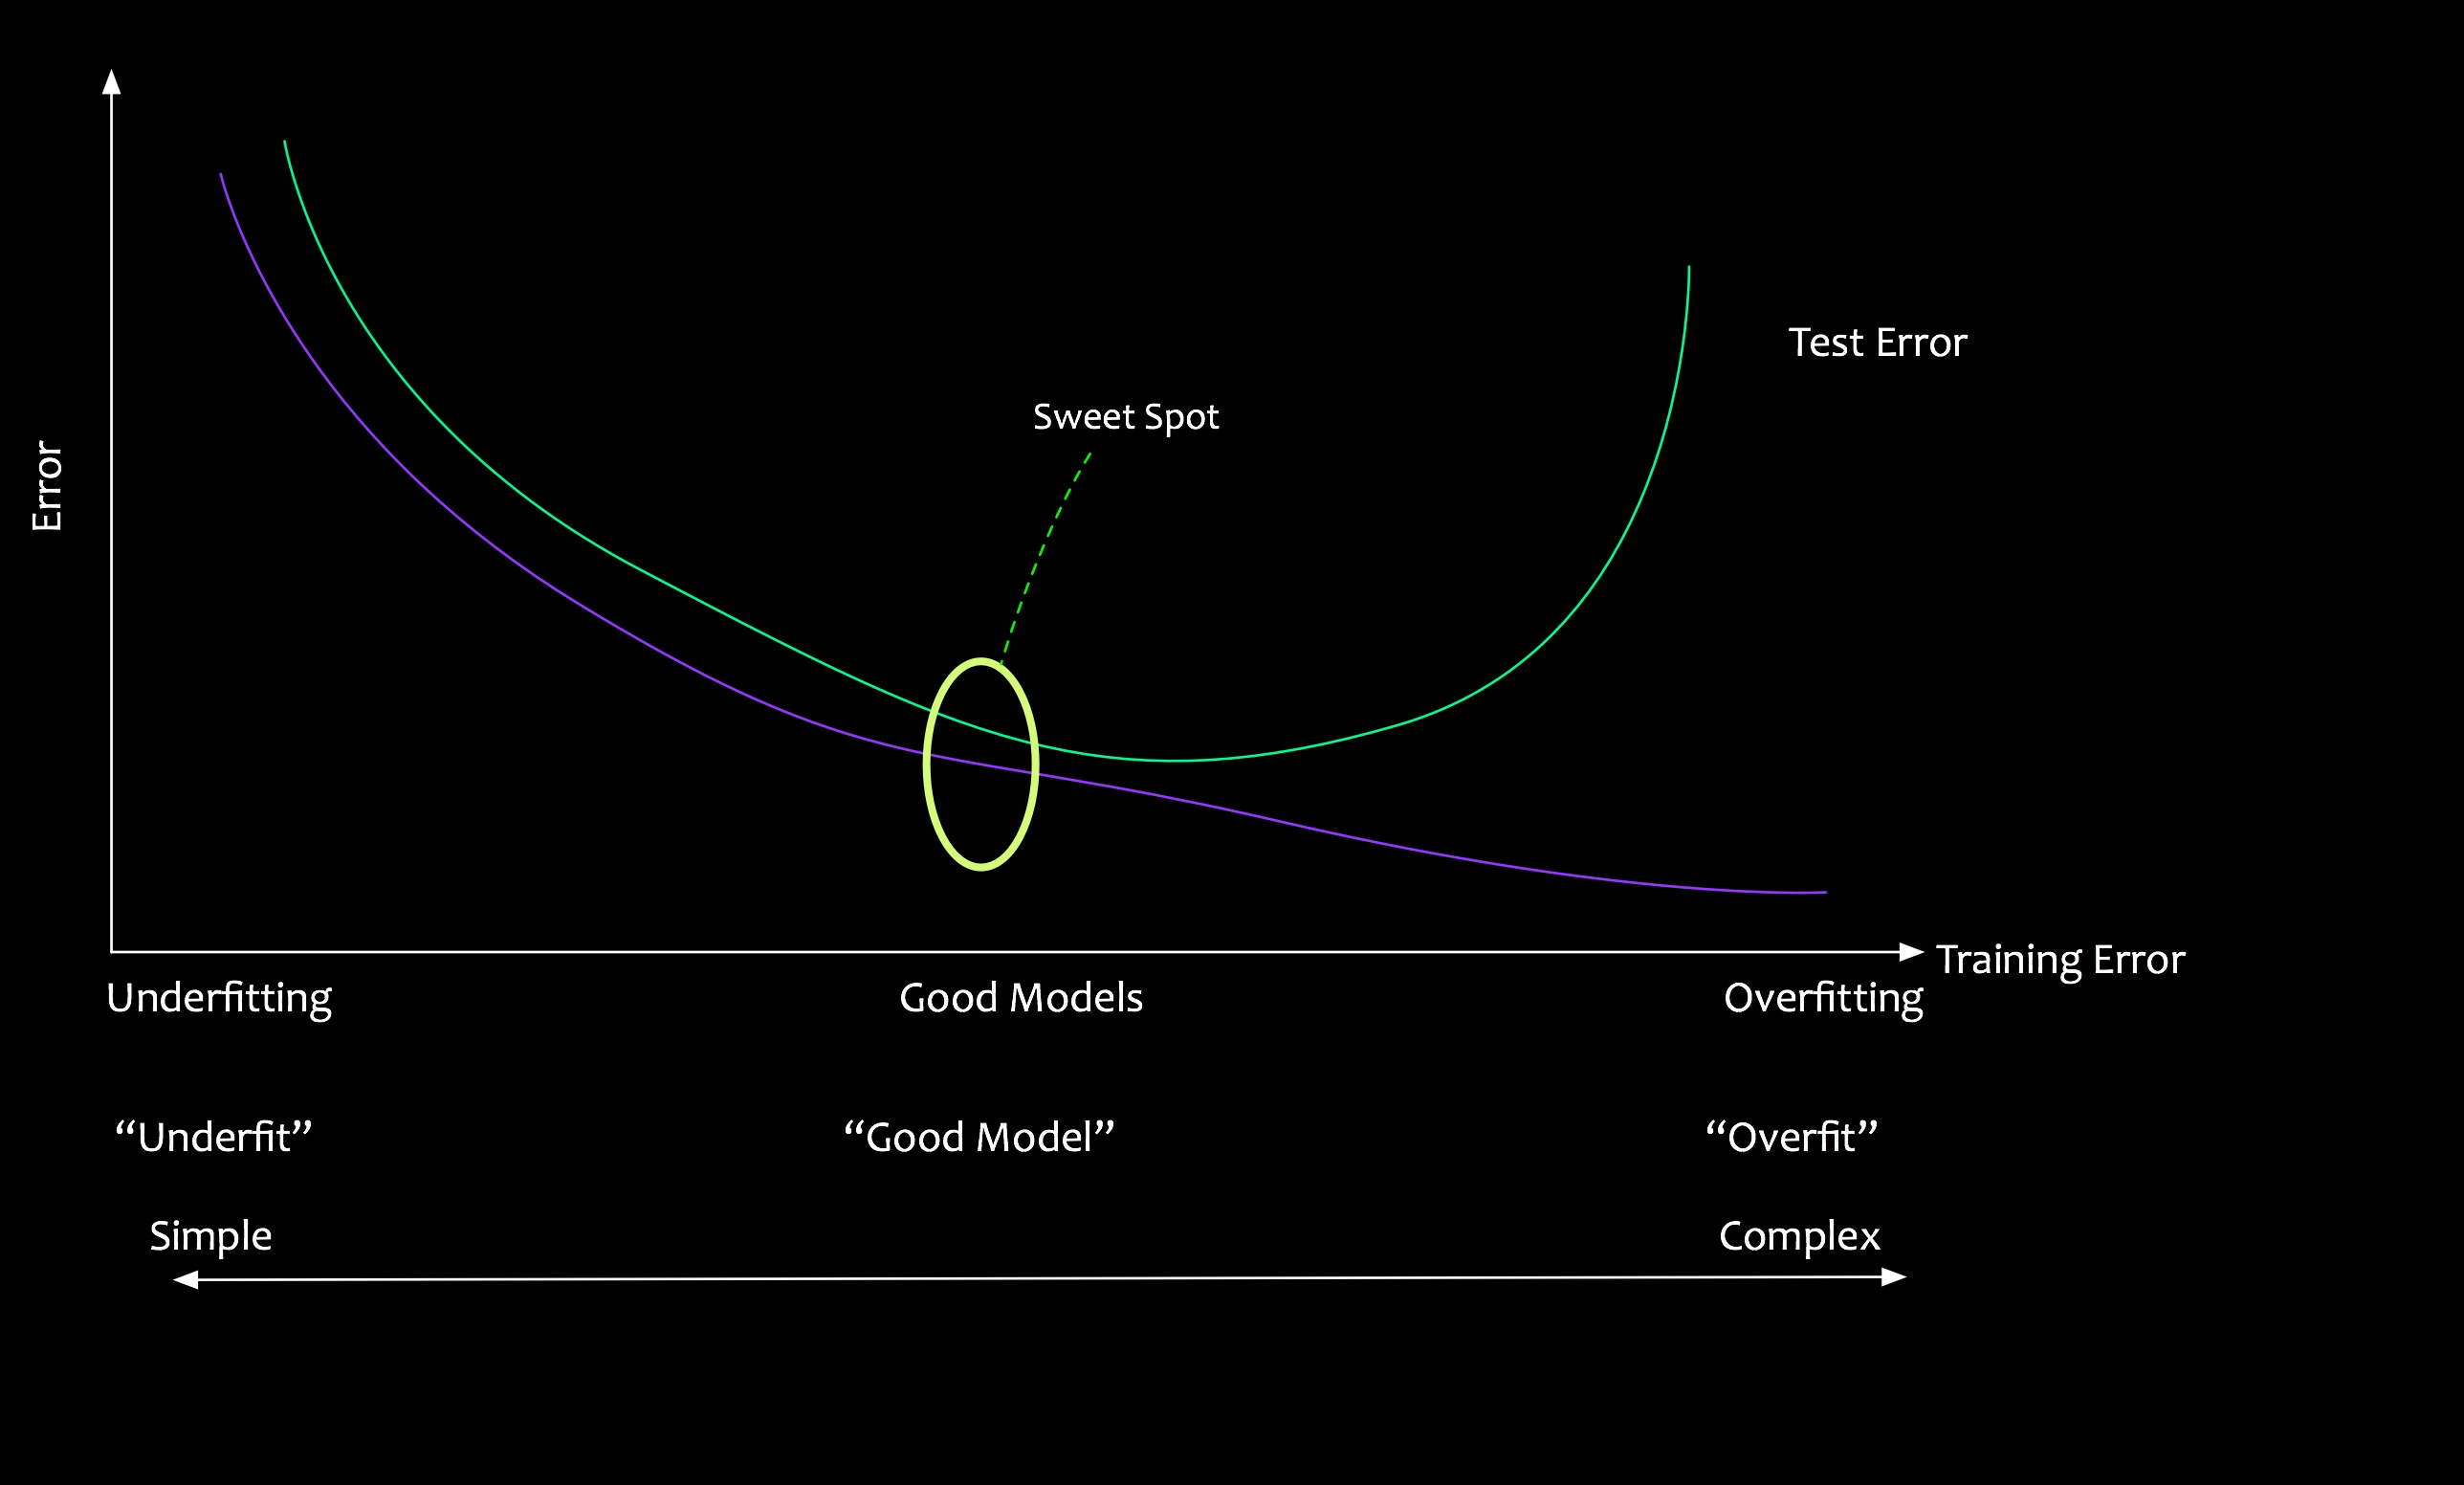
\includegraphics[width=0.8\linewidth,keepaspectratio]{bvmodel}
%\end{center}
%
%\end{frame}



%%%%%%%%%%%%%%%%%%%%%%%%%%%%%%%%%%%%%%%%%%%%%%%%%%%%%%%%%%
\begin{frame}[fragile]\frametitle{Under-fitting vs Over-fitting}
\begin{center}
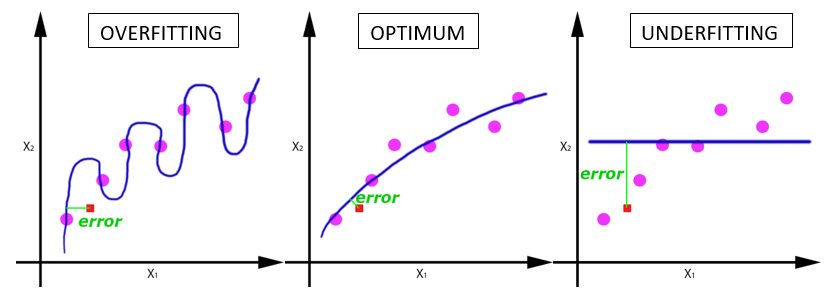
\includegraphics[width=\linewidth,keepaspectratio]{unovfit1}
\end{center}
\tiny{(Reference: What is Machine Learning? - An Introduction- itdadao)}

\end{frame}


%%%%%%%%%%%%%%%%%%%%%%%%%%%%%%%%%%%%%%%%%%%%%%%%%%%%%%%%%%%
%\begin{frame}[fragile]\frametitle{Under-fitting vs Over-fitting}
%\begin{center}
%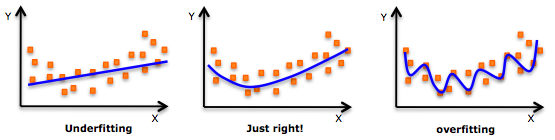
\includegraphics[width=\linewidth,keepaspectratio]{unovfit}
%\end{center}
%
%\end{frame}


%%%%%%%%%%%%%%%%%%%%%%%%%%%%%%%%%%%%%%%%%%%%%%%%%%%%%%%%%%
\begin{frame}[fragile]\frametitle{Over-fitting}
\begin{itemize}
\item Over-fitting: occurs when model ``memorizes'' training data
%\begin{itemize}
%\item very low error rate on training data
%\item yet, high error rate on test data
%\end{itemize}
\item Model does not generalize to the overall problem
\item This is bad! We wish to avoid over-fitting
\item Techniques: Regularization (Penalty) and Drop Out (Neural Network)
\end{itemize}
\end{frame}


%%%%%%%%%%%%%%%%%%%%%%%%%%%%%%%%%%%%%%%%%%%%%%%%%%%%%%%%%%%%%%%%%%%%%%%%
\begin{frame}[fragile]\frametitle{Detection}
Roughly speaking, over-fitting typically occurs when the ratio $\frac{ComplexityOfTheModel}{TrainingSize}$ is too high.

\begin{center}
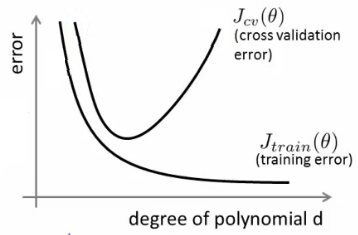
\includegraphics[width=0.4\linewidth,keepaspectratio]{ovefit1}

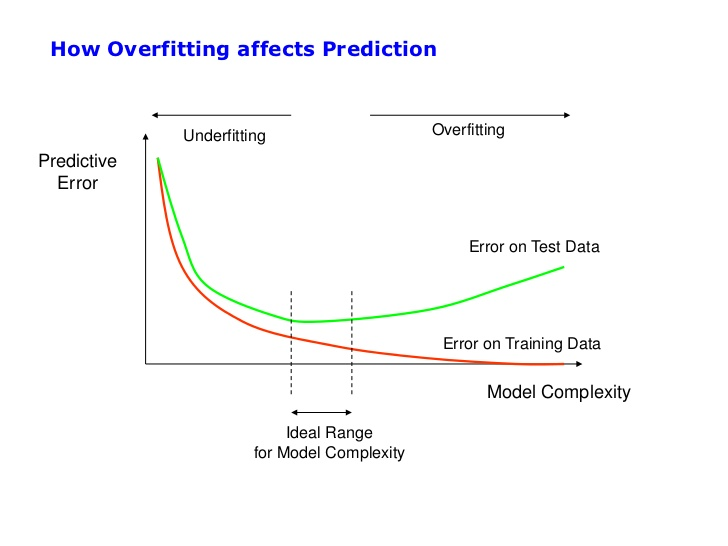
\includegraphics[width=0.4\linewidth,keepaspectratio]{ovefit2}

\end{center}
	\begin{itemize}
	\item If your data is in two dimensions, you have 10000 points in the training set and the model is a line, you are likely to under-fit.
	\item If your data is in two dimensions, you have 10 points in the training set and the model is 100-degree polynomial, you are likely to over-fit. 
	\end{itemize}
	
(Ref:Why Is Over-fitting Bad in Machine Learning? - StackOverflow)
\end{frame}

%%%%%%%%%%%%%%%%%%%%%%%%%%%%%%%%%%%%%%%%%%%%%%%%%%%%%%%%%%%%%%%%%%%%%%%%
\begin{frame}[fragile]\frametitle{Solution}

	\begin{itemize}
	\item In many texts, ``iterations'' is used on X axis, which is easy to imagine in case of Neural Networks, where each epoch refines model by fitting better question/weights.
	\item In case of Machine Learning, there no iterations. How to detect Over-fitting in case of Polynomial Regression?
	\item Initially when, polynomial equation to start with is simple, it has not fit the data yet, so its under fitting phase. Losses are HIGH for both, training as well as testing (validation)
	\item As more levels get added in tree or more degrees in polynomial regression, under-fitting reduces and losses come down.
	\item At one point, training loss still reduces but validation los starts jumping up. Thats over-fitting. Model is fitting training data TOO tightly and is OFF the validation data.
	\end{itemize}
	
(Ref:Why Is Over-fitting Bad in Machine Learning? - StackOverflow)
\end{frame}



% %%%%%%%%%%%%%%%%%%%%%%%%%%%%%%%%%%%%%%%%%%%%%%%%%%%%%%%%%%%%%%%%%%%%%%%%
% \begin{frame}[fragile]\frametitle{Detection}
% Generalization curve: loss for both the training set and validation wrt training iterations.
% \begin{center}
% 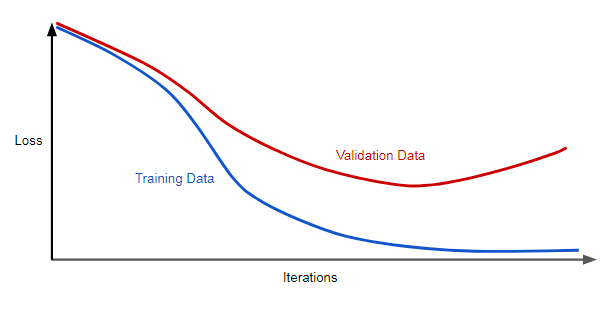
\includegraphics[width=0.4\linewidth,keepaspectratio]{reg1}
% \end{center}
	% \begin{itemize}
	% \item Training loss gradually decreases, 
	% \item but validation loss eventually goes up. 
	% \end{itemize}
	
	% % (Ref: https://developers.google.com/machine-learning/crash-course/regularization-for-simplicity/l2-regularization)
% \end{frame}

% %%%%%%%%%%%%%%%%%%%%%%%%%%%%%%%%%%%%%%%%%%%%%%%%%%%%%%%%%%%%%%%%%%%%%%%%
% \begin{frame}[fragile]\frametitle{Solution}

	% \begin{itemize}
	% \item In over-fitting, during training, as iterations go up, curve fits better and better, it may raise its degree (complexity) higher and higher.
	% \item After some number of iteration, it fits more than needed, becomes far more curvy (complex). When such complex curve is used to test validation data, some points start missing, thus validation error rises after some iterations in over-fitting case.
	% \item Answer is to remove complexity of curve, by reducing, degree.
	% \end{itemize}
	
	% % (Ref: https://developers.google.com/machine-learning/crash-course/regularization-for-simplicity/l2-regularization)
% \end{frame}

%%%%%%%%%%%%%%%%%%%%%%%%%%%%%%%%%%%%%%%%%%%%%%%%%%%%%%%%%%%%%%%%%%%%%%%%
\begin{frame}[fragile]\frametitle{Regularization}
	\begin{itemize}
	\item In regularization, apart from cost function, weighted sum of parameters and features is added
	\item For the features which need to be suppressed, their corresponding coefficient is made large. So their cost component increases
	\item As the Cost needs to be minimized, to reduce these weighted sum, corresponding feature values are reduced, 
	\item So their importances gets lowered dramatically.
	\end{itemize}
\end{frame}



%%%%%%%%%%%%%%%%%%%%%%%%%%%%%%%%%%%%%%%%%%%%%%%%%%%%%%%%%%%%%%%%%%%%%%%%
\begin{frame}[fragile]\frametitle{Regularization}


	\begin{itemize}
	\item Instead of simply aiming to minimize loss (empirical risk minimization): $minimize(Loss(Data|Model))$ 
	\item We'll now minimize loss+complexity, which is called structural risk minimization: $minimize(Loss(Data|Model) + complexity(Model))$
	\end{itemize}
	
	% (Ref: https://developers.google.com/machine-learning/crash-course/regularization-for-simplicity/l2-regularization)
\end{frame}

%%%%%%%%%%%%%%%%%%%%%%%%%%%%%%%%%%%%%%%%%%%%%%%%%%%%%%%%%%%%%%%%%%%%%%%%
\begin{frame}[fragile]\frametitle{Regularization}


	\begin{itemize}
	\item Complexity of model can be represented by many ways, here, Model complexity is taken as a function of the weights of all the features in the model.
	\item Then, a feature weight with a high absolute value is more complex than a feature weight with a low absolute value.
	\end{itemize}
	
	% (Ref: https://developers.google.com/machine-learning/crash-course/regularization-for-simplicity/l2-regularization)
\end{frame}



%%%%%%%%%%%%%%%%%%%%%%%%%%%%%%%%%%%%%%%%%%%%%%%%%%%%%%%%%%
\begin{frame}[fragile]\frametitle{Under-fitting}
\begin{itemize}
\item Under-fitting: occurs when model cannot fit training data well
%\begin{itemize}
%\item very low error rate on training data
%\item very low error rate on test data
%\end{itemize}
\item Model does generalize to the overall problem but not that well
\item This is also bad! We wish to avoid under-fitting
\item Techniques: more features
\end{itemize}
\end{frame}

%%%%%%%%%%%%%%%%%%%%%%%%%%%%%%%%%%%%%%%%%%%%%%%%%%%%%%%%%%%%%%%%%%%%%%%%%%%%%%%%%%
\begin{frame}[fragile]\frametitle{}
\begin{center}
{\Large Bias and Variance}
\end{center}
\end{frame}


%%%%%%%%%%%%%%%%%%%%%%%%%%%%%%%%%%%%%%%%%%%%%%%%%%%%%%%%%%%%%%%%%%%%%%%%%%%%%%%%%%
\begin{frame}[fragile]\frametitle{}
\begin{center}
{\Large Evaluation Metrics: Prediction Bias}
\end{center}
\end{frame}

%%%%%%%%%%%%%%%%%%%%%%%%%%%%%%%%%%%%%%%%%%%%%%%%%%%%%%%%%%
\begin{frame}[fragile]\frametitle{Types of Errors}
The prediction error can be broken down into:
\begin{itemize}
\item Bias Error
\item Variance Error
\end{itemize}
error(X) = noise(X) + bias(X) + variance(X)
\end{frame}

%%%%%%%%%%%%%%%%%%%%%%%%%%%%%%%%%%%%%%%%%%%%%%%%%%%%%%%%%%
\begin{frame}[fragile]\frametitle{Bias}

\begin{itemize}
\item Bias is the simplifying assumption made by a model to make the target function easier to learn.
\item A high bias makes it fast to learn and easier to understand but is generally less flexible.  In turn, it has lower predictive performance on complex problems.
\item 
    Low Bias: Suggests less assumptions about the form of the target function.
    \item
    High-Bias: Suggests more assumptions about the form of the target function.

\end{itemize}
\end{frame}

%%%%%%%%%%%%%%%%%%%%%%%%%%%%%%%%%%%%%%%%%%%%%%%%%%%%%%%%%%
\begin{frame}[fragile]\frametitle{Variance }

\begin{itemize}
\item Variance is the amount that the estimate of the target function will change if different training data was used.
\item  Ideally, it should not change too much from one training dataset to the next, meaning that the algorithm is good at picking out the hidden underlying mapping between the inputs and the output variables.
\item 
    Low Variance: Suggests small changes to the estimate of the target function with changes to the training dataset.
    \item 
    High Variance: Suggests large changes to the estimate of the target function with changes to the training dataset.

\end{itemize}
\end{frame}


% %%%%%%%%%%%%%%%%%%%%%%%%%%%%%%%%%%%%%%%%%%%%%%%%%%%%%%%%%%%%%%%%%%%%%%%%
% \begin{frame}[fragile]\frametitle{Prediction Bias}

% \begin{itemize}
% \item Logistic Regression predictions should be unbiased.
% \item average of predictions == average of observations (actuals)
% \item If they are not equal, we say that there is a bias.
% \item If bias is 0, then both, predications and actuals match.
% \item Zero bias alone does not mean everything in your system is perfect.
% \item This being comparison of averages, your actual values can fly anywhere, but the average comes ok.
% \item But it's a great sanity check.
% \end{itemize}


% % (Ref: https://developers.google.com/machine-learning/crash-course/classification/video-lecture)
% \end{frame}


% %%%%%%%%%%%%%%%%%%%%%%%%%%%%%%%%%%%%%%%%%%%%%%%%%%%%%%%%%%%%%%%%%%%%%%%%
% \begin{frame}[fragile]\frametitle{Prediction Bias}

% \begin{itemize}
% \item If you have bias, you have a problem.
% \begin{itemize}
% \item Incomplete feature set?
% \item Buggy pipeline?
% \item Biased training sample?
% \end{itemize}
% \item Don't fix bias with a calibration layer, fix it in the model.
% \item Look for bias in slices of data -- this can guide improvements
% \end{itemize}


% % (Ref: https://developers.google.com/machine-learning/crash-course/classification/video-lecture)
% \end{frame}


% %%%%%%%%%%%%%%%%%%%%%%%%%%%%%%%%%%%%%%%%%%%%%%%%%%%%%%%%%%%%%%%%%%%%%%%%
% \begin{frame}[fragile]\frametitle{Prediction Bias}
% How to check? Calibration plot
% \begin{itemize}
% \item Make some data bins.
% \item Compare, average predictions and actuals. Calculate bias.
% \item Are they shooting off the band?
% \end{itemize}
% \begin{center}
% 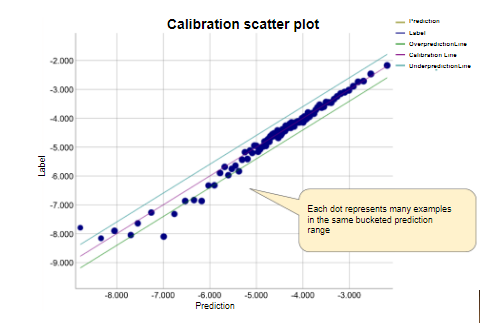
\includegraphics[width=0.6\linewidth]{logistic5}
% \end{center}


% % (Ref: https://developers.google.com/machine-learning/crash-course/classification/video-lecture)
% \end{frame}


%%%%%%%%%%%%%%%%%%%%%%%%%%%%%%%%%%%%%%%%%%%%%%%%%%%%%%%%%%%%%%%%%%%%%%%%
\begin{frame}[fragile]\frametitle{Intuition: Example}
	\begin{itemize}
	\item We have collected past observations of Mice's Heights and Weights.
	\item Clearly,the relationship is sort of curved.
	\item Wish to predict Height given Weight.
	\item Different algorithms will have different underlying structures to fit this regression data.
	\end{itemize}
	
\begin{center}
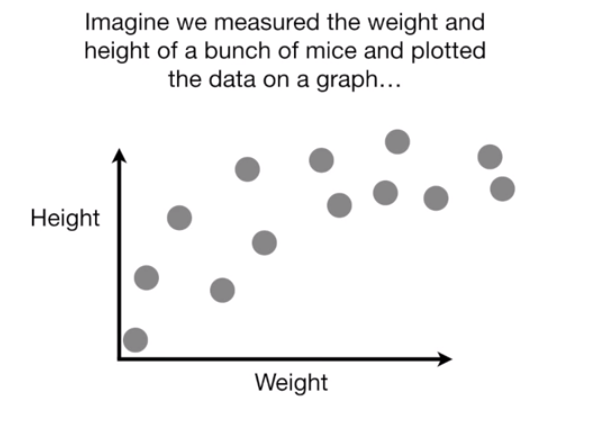
\includegraphics[width=0.4\linewidth,keepaspectratio]{bv1}
\end{center}
	
\tiny{(Ref: Machine Learning Fundamentals: Bias and Variance -StatQuest with Josh Starmer )}
\end{frame}

%%%%%%%%%%%%%%%%%%%%%%%%%%%%%%%%%%%%%%%%%%%%%%%%%%%%%%%%%%%%%%%%%%%%%%%%
\begin{frame}[fragile]\frametitle{Intuition: True Relationship}
	\begin{itemize}
	\item We have collected past observations of Mice's Heights and Weights.
	\item Clearly,the relationship is sort of curved.
	\item Different algorithms will have different underlying structures to fit this regression data.
	\end{itemize}
	
\begin{center}
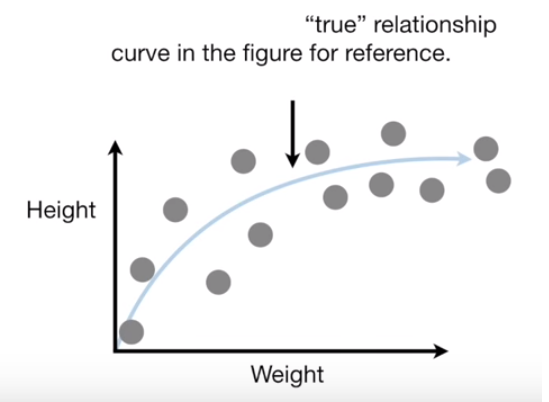
\includegraphics[width=0.4\linewidth,keepaspectratio]{bv2}
\end{center}
	
\tiny{(Ref: Machine Learning Fundamentals: Bias and Variance -StatQuest with Josh Starmer )}
\end{frame}

%%%%%%%%%%%%%%%%%%%%%%%%%%%%%%%%%%%%%%%%%%%%%%%%%%%%%%%%%%%%%%%%%%%%%%%%
\begin{frame}[fragile]\frametitle{Intuition: Machine Learning}
	\begin{itemize}
	\item Split data into training and testing (validation)
	\item Blue for training
	\item Green for testing
	\end{itemize}
	
\begin{center}
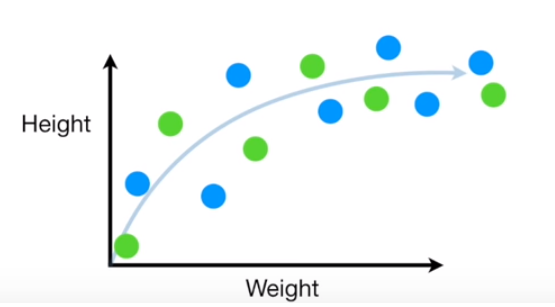
\includegraphics[width=0.4\linewidth,keepaspectratio]{bv3}
\end{center}
	
\tiny{(Ref: Machine Learning Fundamentals: Bias and Variance -StatQuest with Josh Starmer )}
\end{frame}

%%%%%%%%%%%%%%%%%%%%%%%%%%%%%%%%%%%%%%%%%%%%%%%%%%%%%%%%%%%%%%%%%%%%%%%%
\begin{frame}[fragile]\frametitle{Intuition: Linear Regression}
	\begin{itemize}
	\item Fitting Linear Regression model on the training data (blue dots)
	\item It fits a line, whatever the underlying data is.
	\item But it finds best line that minimizes Least Square error.
	\item Anyway, it can not bend, so said to have HIGH bias. It is not very accurate.
	\item Inability of Machine Learning model to capture the TRUE relationship is called as {\bf Bias}.
	\end{itemize}
	
\begin{center}
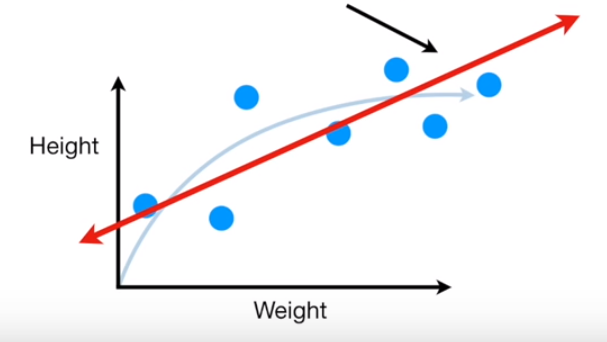
\includegraphics[width=0.4\linewidth,keepaspectratio]{bv4}
\end{center}
	
\tiny{(Ref: Machine Learning Fundamentals: Bias and Variance -StatQuest with Josh Starmer )}
\end{frame}

%%%%%%%%%%%%%%%%%%%%%%%%%%%%%%%%%%%%%%%%%%%%%%%%%%%%%%%%%%%%%%%%%%%%%%%%
\begin{frame}[fragile]\frametitle{Intuition: Non-Linear (Tree) Regression}
	\begin{itemize}
	\item Some other Machine Learning model can give high degree and flexible model.
	\item As it passes through points, its very accurate (as there is just no error)
	\item Being flexible, it has ability to represent true relationship, so very little bias.
	\end{itemize}
	
\begin{center}
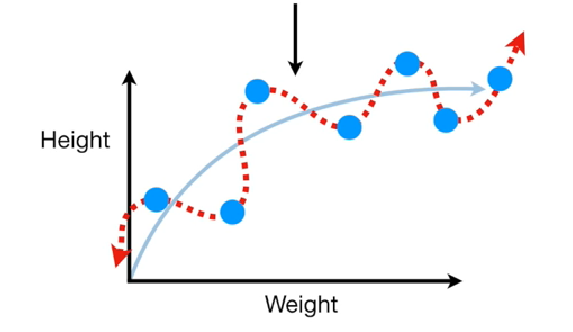
\includegraphics[width=0.4\linewidth,keepaspectratio]{bv5}
\end{center}
	
\tiny{(Ref: Machine Learning Fundamentals: Bias and Variance -StatQuest with Josh Starmer )}
\end{frame}

%%%%%%%%%%%%%%%%%%%%%%%%%%%%%%%%%%%%%%%%%%%%%%%%%%%%%%%%%%%%%%%%%%%%%%%%
\begin{frame}[fragile]\frametitle{Intuition: Training set Comparison}
	\begin{itemize}
	\item Linear model has error on Training set. High Bias.
	\item Non-linear model has almost no error on Training set. Low Bias.
	\end{itemize}
	
\begin{center}
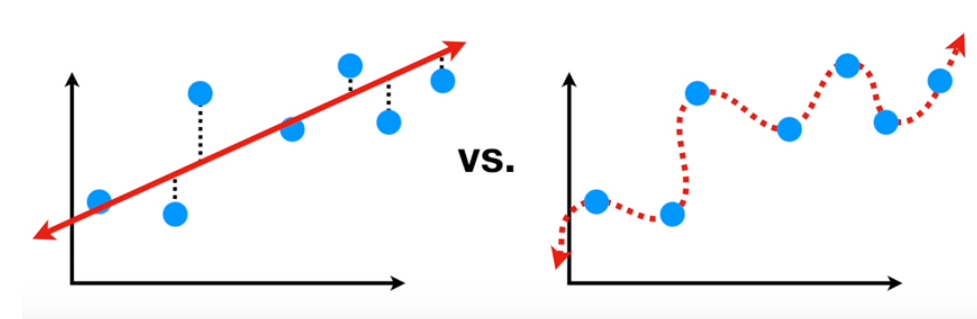
\includegraphics[width=0.7\linewidth,keepaspectratio]{bv6}
\end{center}
	
\tiny{(Ref: Machine Learning Fundamentals: Bias and Variance -StatQuest with Josh Starmer )}
\end{frame}

%%%%%%%%%%%%%%%%%%%%%%%%%%%%%%%%%%%%%%%%%%%%%%%%%%%%%%%%%%%%%%%%%%%%%%%%
\begin{frame}[fragile]\frametitle{Intuition: Testing set Comparison}
	\begin{itemize}
	\item When same model is applied on the testing set, how does it fair?
	\item Which model looks better? Linear or Non-Linear?
	\item Linear is not accurate, but the Non-linear is far too bad.
	\item This is called as {\bf Variance}.
	\item Difference in fits on different datasets is the Variance.
	\item Linear model has less Variance and Non Linear model has High Variance.
	\end{itemize}
	
\begin{center}
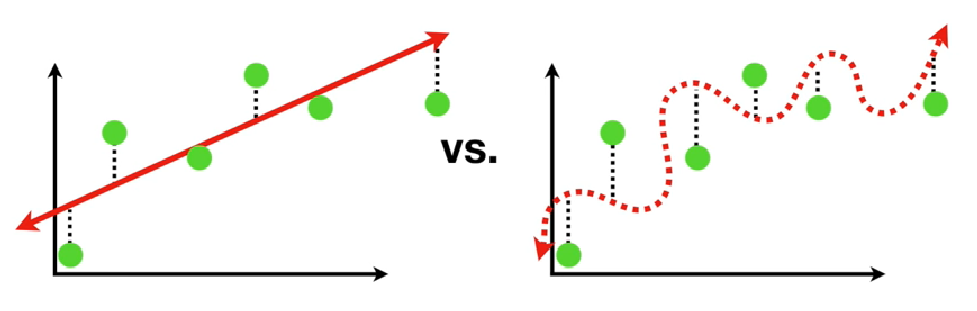
\includegraphics[width=0.7\linewidth,keepaspectratio]{bv7}
\end{center}
	
\tiny{(Ref: Machine Learning Fundamentals: Bias and Variance -StatQuest with Josh Starmer )}
\end{frame}

%%%%%%%%%%%%%%%%%%%%%%%%%%%%%%%%%%%%%%%%%%%%%%%%%%%%%%%%%%%%%%%%%%%%%%%%
\begin{frame}[fragile]\frametitle{Intuition: Ideal}
	\begin{itemize}
	\item Linear model gives good predictions but not great predictions, but its consistent.
	\item Non linear model gives great predictions but not consistent many a times.
	\item Ideal model captures underlying true relationship. So, low Bias and low Variance.
	\item It is done by finding a Sweet spot between simple model and complex model.
	\item 3 such methods of finding sweet spot are : regularization, bagging and boosting.
	\end{itemize}
	
\begin{center}
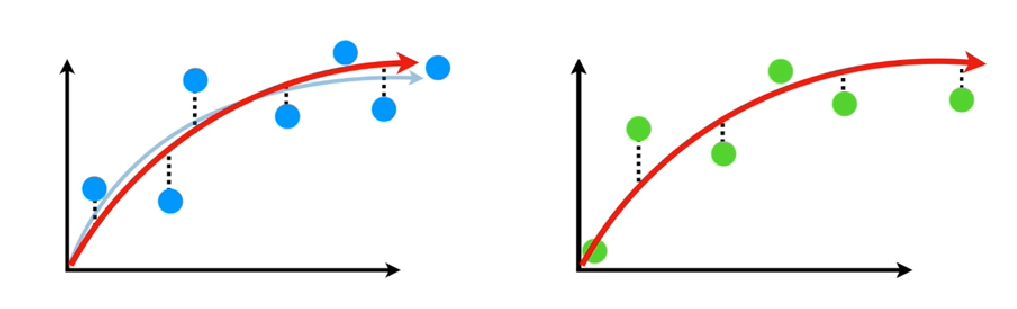
\includegraphics[width=0.7\linewidth,keepaspectratio]{bv8}
\end{center}
	
\tiny{(Ref: Machine Learning Fundamentals: Bias and Variance -StatQuest with Josh Starmer )}
\end{frame}



%%%%%%%%%%%%%%%%%%%%%%%%%%%%%%%%%%%%%%%%%%%%%%%%%%%%%%%%%
\begin{frame}[fragile]\frametitle{Bias and Variance (Recap)}
\begin{itemize}
\item Bias: the error introduced by modeling for complex situation by a much simpler model
\item {\bf The more flexible (complex) a method is, the less bias it will generally have.}
\item Variance: how much the learned model will change if the training set was different 
\item Does changing a few observations in the training set, dramatically affect the model?
\item {\bf Generally, the more flexible (complex) a method is, the more variance it has.}
\end{itemize}
\end{frame}


%%%%%%%%%%%%%%%%%%%%%%%%%%%%%%%%%%%%%%%%%%%%%%%%%%%%%%%%%
\begin{frame}[fragile]\frametitle{Learning Method Bias}
\begin{itemize}
\item Bias: the error introduced by modeling a real-life problem (usually extremely complicated) by a much simpler model.
\item High bias is a strong view of modeling with simplistic solution.

\begin{itemize}
\item Example: linear regression assumes a linear relationship between the target variable Y and the predictor variables X
\item It's unlikely that the relationship is exactly linear, so some bias will be present in the model
\end{itemize}
\item The more flexible (complex) a method is, the less bias it will generally have.

\end{itemize}
\end{frame}

%%%%%%%%%%%%%%%%%%%%%%%%%%%%%%%%%%%%%%%%%%%%%%%%%%%%%%%%%
\begin{frame}[fragile]\frametitle{Learning Method Variance}
\begin{itemize}
\item Variance: how much the learned model will change if the training set was different 
\begin{itemize}
\item Does changing a few observations in the training set, dramatically affect the model?
\item Ideally, answer is no.
\end{itemize}
\item Generally, the more flexible (complex) a method is, the more variance it has.
\end{itemize}
\end{frame}

%%%%%%%%%%%%%%%%%%%%%%%%%%%%%%%%%%%%%%%%%%%%%%%%%%%%%%%%%%
\begin{frame}[fragile]\frametitle{Example }

\begin{itemize}
\item Imagine you have 5 training datasets of the same problem
\item Imagine using an machine learning algo on these sets, so we have 5 models
\item High bias algo gives off the mark result
\item Low variance gives converged results
\item Low bias algo gives towards the mark result
\item High variance gives spread results
\end{itemize}
\begin{center}
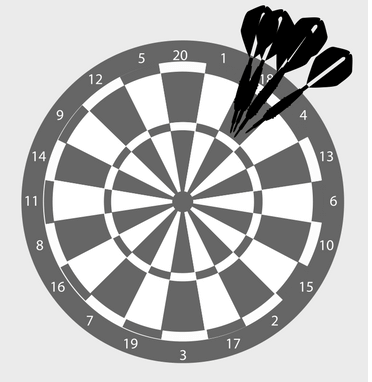
\includegraphics[width=0.3\linewidth,keepaspectratio]{hblv}
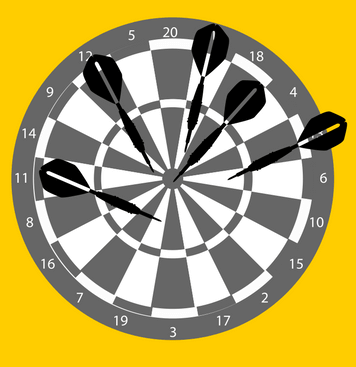
\includegraphics[width=0.3\linewidth,keepaspectratio]{hvlb}
\end{center}

\end{frame}

% %%%%%%%%%%%%%%%%%%%%%%%%%%%%%%%%%%%%%%%%%%%%%%%%%%%
% \begin{frame}[fragile] \frametitle{Bias vs Variations}

% %\adjustbox{valign=t}{
% %\begin{minipage}{0.4\linewidth}
% %\begin{center}
% %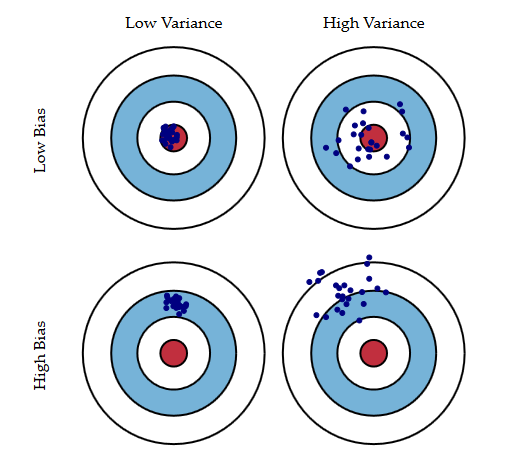
\includegraphics[width=0.4\linewidth,keepaspectratio]{biasvariations}
% %\end{center}
% %%
% %\end{minipage}
% %}
% %\hfill
% %\adjustbox{valign=t}{
% %\begin{minipage}{0.45\linewidth}
% \begin{itemize}
% \item Bias: the difference 
% between expected 
% (average) prediction of the 
% model and the correct 
% value. 
% \item Variance: how the 
% predictions for a given point 
% vary between different 
% realizations for the model. 
% \end{itemize}
% %
% %\end{minipage}
% %}
% %{\tiny http://scott.fortmann-roe.com/docs/BiasVariance.html }
% \end{frame}

%%%%%%%%%%%%%%%%%%%%%%%%%%%%%%%%%%%%%%%%%%%%%%%%%%%
\begin{frame}[fragile] \frametitle{Bias vs Variations}

%\adjustbox{valign=t}{
%\begin{minipage}{0.4\linewidth}
\begin{center}
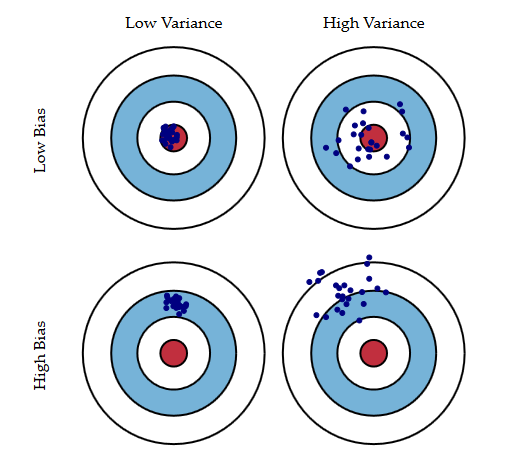
\includegraphics[width=0.6\linewidth,keepaspectratio]{biasvariations}
\end{center}
{\tiny http://scott.fortmann-roe.com/docs/BiasVariance.html }
%
%\end{minipage}
%}
%\hfill
%\adjustbox{valign=t}{
%\begin{minipage}{0.45\linewidth}
%\begin{itemize}
%\item Bias: the difference 
%between expected 
%(average) prediction of the 
%model and the correct 
%value. 
%\item Variance: how the 
%predictions for a given point 
%vary between different 
%realizations for the model. 
%\end{itemize}
%
%\end{minipage}
%}
{\tiny http://scott.fortmann-roe.com/docs/BiasVariance.html }
\end{frame}

% %%%%%%%%%%%%%%%%%%%%%%%%%%%%%%%%%%%%%%%%%%%%%%%%%%%%%%%%%%
% \begin{frame}[fragile]\frametitle{Example}
% \begin{itemize}
% \item Raj, a seven-year-old kid, was just introduced to the concept of multiplication. He had mastered the tables of 1 and 2. His next challenge was to learn the table of 3. He was very excited and started to practice the multiplication table of 3. His table is something like this:
% \begin{lstlisting}
    % 3 x 1 = 4
    % 3 x 2 = 7
    % 3 x 3 = 10
    % 3 x 4 = 13
    % 3 x 5 = 16
% \end{lstlisting}
% \item Taj, Raj's classmate, was on the same boat. His table looked something like this:
% \begin{lstlisting}
    % 3 x 1 = 5
    % 3 x 2 = 9
    % 3 x 3 = 18
    % 3 x 4 = 24
    % 3 x 5 = 30
% \end{lstlisting}
% \end{itemize}
% \end{frame}

% %%%%%%%%%%%%%%%%%%%%%%%%%%%%%%%%%%%%%%%%%%%%%%%%%%%%%%%%%%
% \begin{frame}[fragile]\frametitle{Understanding the models}
% \begin{itemize}
% \item Raj's model has an invalid assumption. 
% \item It assumes that the operation of multiplication implies to add one after the result. 
% \item This assumption introduces the bias error. 
% \item The assumption is consistent i.e. add 1 to the output. 
% \item This means that Raj's model has a low bias.
% \end{itemize}
% \end{frame}

% %%%%%%%%%%%%%%%%%%%%%%%%%%%%%%%%%%%%%%%%%%%%%%%%%%%%%%%%%%
% \begin{frame}[fragile]\frametitle{Understanding the models}
% \begin{itemize}
% \item Raj's model results in output that is consistently 1 number away from the actual. 
% \item This means that his model has a low variance.
% \end{itemize}
% \end{frame}

% %%%%%%%%%%%%%%%%%%%%%%%%%%%%%%%%%%%%%%%%%%%%%%%%%%%%%%%%%%
% \begin{frame}[fragile]\frametitle{Understanding the models}
% \begin{itemize}
% \item Taj's model's output is all over the place. 
% \item His model outputs deviates a lot from the actual value. 
% \item There is no consistent pattern for deviation. 
% \item Taj's model has high bias and high variation.
% \end{itemize}
% \end{frame}
%
%%%%%%%%%%%%%%%%%%%%%%%%%%%%%%%%%%%%%%%%%%%%%%%%%%%%%%%%%%
%\begin{frame}[fragile]\frametitle{Bias-Variance Trade-Off}
%\begin{itemize}
%\item Expected test set error can be decomposed into the sum of the model's variance, it's squared bias, and the variance of its error terms.
%\begin{center}
%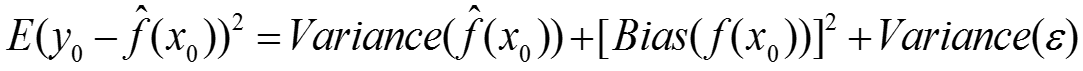
\includegraphics[width=\linewidth,keepaspectratio]{biasvar}
%\end{center}
%\item As a statistical method gets more complex, the bias will decrease and the variance will increase.
%\item Expected error on the test set may go up or down.
%\end{itemize}
%\end{frame}
%
%




%%%%%%%%%%%%%%%%%%%%%%%%%%%%%%%%%%%%%%%%%%%%%%%%%%%%%%%%%%
%\begin{frame}[fragile]\frametitle{Bias-Variance Trade-Off Example}
%\begin{center}
%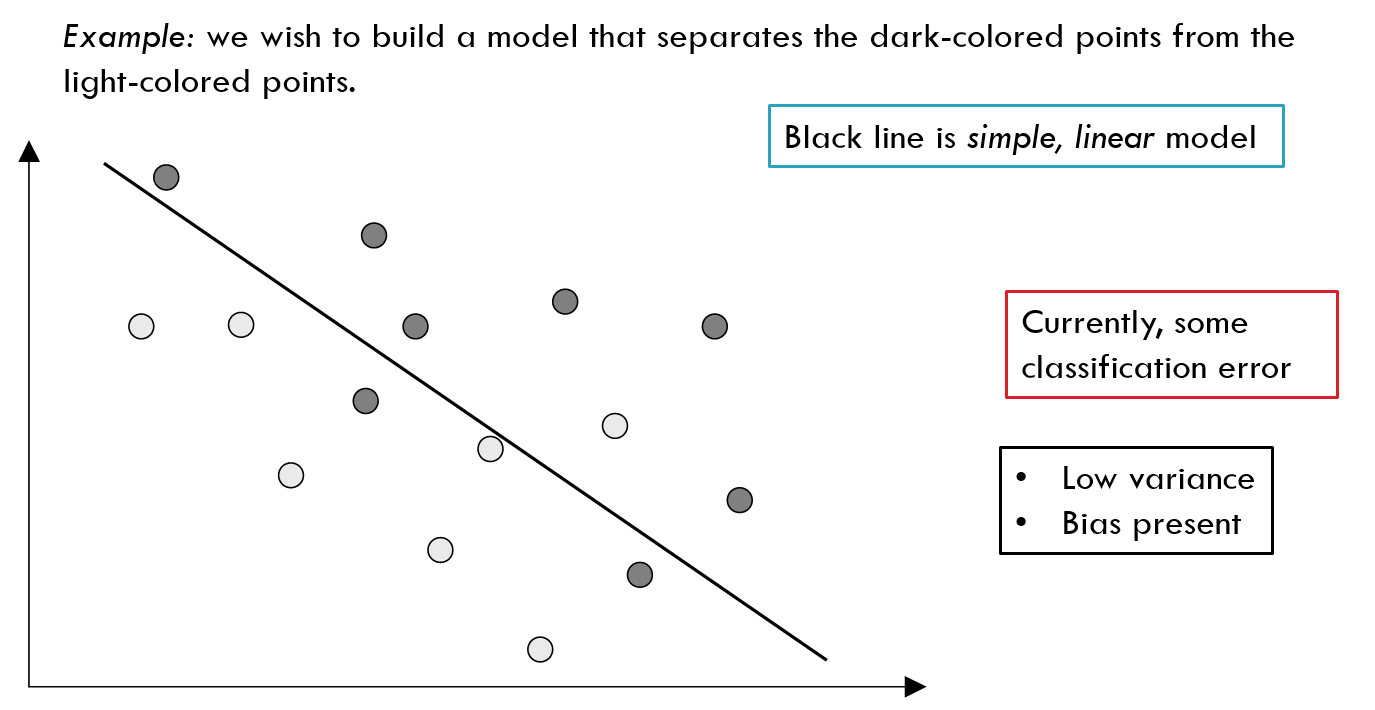
\includegraphics[width=\linewidth,keepaspectratio]{errex}
%\end{center}
%\end{frame}
%
%%%%%%%%%%%%%%%%%%%%%%%%%%%%%%%%%%%%%%%%%%%%%%%%%%%%%%%%%%
%\begin{frame}[fragile]\frametitle{Bias-Variance Trade-Off Example}
%\begin{center}
%\includegraphics[width=\linewidth,keepaspectratio]{errex1}
%\end{center}
%\end{frame}
%
%%%%%%%%%%%%%%%%%%%%%%%%%%%%%%%%%%%%%%%%%%%%%%%%%%%%%%%%%%
%\begin{frame}[fragile]\frametitle{Bias-Variance Trade-Off Example}
%\begin{center}
%\includegraphics[width=\linewidth,keepaspectratio]{errex2}
%\end{center}
%\end{frame}

%%%%%%%%%%%%%%%%%%%%%%%%%%%%%%%%%%%%%%%%%%%%%%%%%%%%%%%%%%%%
%%\begin{frame}[fragile]\frametitle{Model Generalization}
%%\begin{itemize}
%%\item Learning too much from dataset is overfitting. 
%%\item Not generalized the learning to be useful to unseen data.
%%\item On the other end, learning too little results in underfitting. Can't even learn from the given data.
%%\item Summary:
%%\begin{itemize}
%%\item A model that overfits it complex. It performs very well on training data. It performs poorly on testing data.
%%\item A model that underfits is too simplistic. It doesn't perform will on both training and testing data.
%%\item A good model balances underfitting and overfitting. It generalizes well. It is as simple as possible but no simpler.
%%\end{itemize}
%%\item This balancing act is called bias-variance trade-off.
%%\end{itemize}
%%\end{frame}
%%
%%
%%
%%%%%%%%%%%%%%%%%%%%%%%%%%%%%%%%%%%%%%%%%%%%%%%%%%%%%%%%%%%%
%%\begin{frame}[fragile]\frametitle{Model Overfitting}
%%\begin{itemize}
%%\item Errors committed by a classification model are generally divided into:
%%\begin{itemize}
%%\item Training errors: misclassification on training set records
%%\item Generalization errors (testing errors): errors made on testing set / previously unseen instances
%%\end{itemize}
%%\item Good model has low training and low generalization error.
%%\item Overfitting: model has low training error rate, but high generalization errors
%%
%%\item Reasons for Overfitting
%%\begin{itemize}
%%\item Presence of noise
%%\item Lack of representative samples
%%\end{itemize}
%%\end{itemize}
%%\end{frame}

%%%%%%%%%%%%%%%%%%%%%%%%%%%%%%%%%%%%%%%%%%%%%%%%%%%%
%\begin{frame}[fragile] \frametitle{Model Underfitting and Overfitting}
%
%\adjustbox{valign=t}{
%\begin{minipage}{0.4\linewidth}
%\begin{center}
%\includegraphics[width=\linewidth,keepaspectratio]{unov}
%\end{center}
%
%\end{minipage}
%}
%\hfill
%\adjustbox{valign=t}{
%\begin{minipage}{0.45\linewidth}
%\small
%\begin{itemize}
%\item When tree is small:
%\begin{itemize}
%\item Underfitting
%\item Large training error rate
%\item Large testing error rate
%\item Structure of data isn't yet learned
%\end{itemize}
%\item When tree gets too large:
%\begin{itemize}
%\item Beware of overfitting
%\item Training error rate decreases while testing error rate increases
%\item Tree is too complex
%\end{itemize}
%\end{itemize}
%
%\end{minipage}
%}
%\end{frame}

% %%%%%%%%%%%%%%%%%%%%%%%%%%%%%%%%%%%%%%%%%%%%%%%%%%%%%%%%%%%%%%%%%%%%%%%%%%%%%%%%%%
% \begin{frame}[fragile]\frametitle{}
% \begin{center}
% {\Large Machine Learning Model Errors - Mathematically}
% \end{center}
% \end{frame}


% %%%%%%%%%%%%%%%%%%%%%%%%%%%%%%%%%%%%%%%%%%%%%%%%%%%%%%%%%%
% \begin{frame}[fragile]\frametitle{Error Properties}
% \begin{itemize}
% \item True value of the target variable is the sum of a deterministic function $f(x)$ and random error $\epsilon$ :  $y = f\left(\textbf{x}\right) + \epsilon$
% \item Error is normally distributed with zero mean and some variance: $\epsilon \sim \mathcal{N}\left(0, \sigma^2\right)$
% \item True value of the target variable is also normally distributed: $y \sim \mathcal{N}\left(f\left(\textbf{x}\right), \sigma^2\right)$
% \end{itemize}
% \end{frame}


% %%%%%%%%%%%%%%%%%%%%%%%%%%%%%%%%%%%%%%%%%%%%%%%%%%%%%%%%%%
% \begin{frame}[fragile]\frametitle{Error Properties}
% The error at the point $x$ decomposes as follows:


% $
% \begin{array}{rcl} 
% \text{Err}\left(\textbf{x}\right) &=& \mathbb{E}\left[\left(y - \widehat{f}\left(\textbf{x}\right)\right)^2\right] \\
% &=& \mathbb{E}\left[y^2\right] + \mathbb{E}\left[\left(\widehat{f}\left(\textbf{x}\right)\right)^2\right] - 2\mathbb{E}\left[y\widehat{f}\left(\textbf{x}\right)\right] \\
% &=& \mathbb{E}\left[y^2\right] + \mathbb{E}\left[\widehat{f}^2\right] - 2\mathbb{E}\left[y\widehat{f}\right] \\
% \end{array}
% $


% (For clarity, we will omit the notation of the argument of the functions.)

% Using formula $\text{Var}\left(z\right) = \mathbb{E}\left[z^2\right] - \mathbb{E}\left[z\right]^2$  or   $\mathbb{E}\left[z\right]^2 = \text{Var}\left(z\right) + \mathbb{E}\left[z^2\right]$ transform above equation to 


% $
% \begin{array}{rcl} 
% \mathbb{E}\left[y^2\right] &=& \text{Var}\left(y\right) + \mathbb{E}\left[y\right]^2 = \sigma^2 + f^2\\
% \mathbb{E}\left[\widehat{f}^2\right] &=& \text{Var}\left(\widehat{f}\right) + \mathbb{E}\left[\widehat{f}\right]^2 \\
% \end{array}
% $


% \end{frame}

% %%%%%%%%%%%%%%%%%%%%%%%%%%%%%%%%%%%%%%%%%%%%%%%%%%%%%%%%%%
% \begin{frame}[fragile]\frametitle{Error Properties}
% By definition, variance is expected value of difference square:

% $
% \begin{array}{rcl} 
% \text{Var}\left(y\right) &=& \mathbb{E}\left[\left(y - \mathbb{E}\left[y\right]\right)^2\right] \\
% &=& \mathbb{E}\left[\left(y - f\right)^2\right] \\
% &=& \mathbb{E}\left[\left(f + \epsilon - f\right)^2\right] \\
% &=& \mathbb{E}\left[\epsilon^2\right] = \sigma^2
% \end{array}
% $

% $\mathbb{E}[y] = \mathbb{E}[f + \epsilon] = \mathbb{E}[f] + \mathbb{E}[\epsilon] = f$
% \end{frame}


% %%%%%%%%%%%%%%%%%%%%%%%%%%%%%%%%%%%%%%%%%%%%%%%%%%%%%%%%%%
% \begin{frame}[fragile]\frametitle{Error Properties}
% And finally, we get to the last term in the sum (original equation). Recall that the error and the target variable are independent of each other:
% $
% \begin{array}{rcl} 
% \mathbb{E}\left[y\widehat{f}\right] &=& \mathbb{E}\left[\left(f + \epsilon\right)\widehat{f}\right] \\
% &=& \mathbb{E}\left[f\widehat{f}\right] + \mathbb{E}\left[\epsilon\widehat{f}\right] \\
% &=& f\mathbb{E}\left[\widehat{f}\right] + \mathbb{E}\left[\epsilon\right] \mathbb{E}\left[\widehat{f}\right]  = f\mathbb{E}\left[\widehat{f}\right]
% \end{array}
% $

% Finally, let's bring this all together:

% $
% \begin{array}{rcl} 
% \text{Err}\left(\textbf{x}\right) &=& \mathbb{E}\left[\left(y - \widehat{f}\left(\textbf{x}\right)\right)^2\right] \\
% &=& \sigma^2 + f^2 + \text{Var}\left(\widehat{f}\right) + \mathbb{E}\left[\widehat{f}\right]^2 - 2f\mathbb{E}\left[\widehat{f}\right] \\
% &=& \left(f - \mathbb{E}\left[\widehat{f}\right]\right)^2 + \text{Var}\left(\widehat{f}\right) + \sigma^2 \\
% &=& \text{Bias}\left(\widehat{f}\right)^2 + \text{Var}\left(\widehat{f}\right) + \sigma^2
% \end{array}
% $
% \end{frame}


% %%%%%%%%%%%%%%%%%%%%%%%%%%%%%%%%%%%%%%%%%%%%%%%%%%%%%%%%%%
% \begin{frame}[fragile]\frametitle{Error Properties}
% the last formula tells us that the forecast error of any model of type $y = f\left(\textbf{x}\right) + \epsilon$ is composed of:

% \begin{itemize}
% \item Squared bias: $\text{Bias}\left(\widehat{f}\right)$ is the average error for all sets of data.
% \item Variance: $\text{Var}\left(\widehat{f}\right)$ is error variability, or by how much error will vary if we train the model on different sets of data;
% \item Irremovable error: $\sigma^2$
% \end{itemize}

% While we cannot do anything with the $\sigma^2$ term, we can influence the first two, as seen before.
% \end{frame}





% %%%%%%%%%%%%%%%%%%%%%%%%%%%%%%%%%%%%%%%%%%%%%%%%%%%%%%%%%%%%%%%%%%%%%%%%%%%%%%%%%%
% \begin{frame}[fragile]\frametitle{}
% \begin{center}
% {\Large Machine Learning Model Errors - On a Lighter Note}
% \end{center}
% \end{frame}



%%%%%%%%%%%%%%%%%%%%%%%%%%%%%%%%%%%%%%%%%%%%%%%%%%%%%%%%%%
\begin{frame}[fragile]\frametitle{On a Lighter Note (Don't start imagining the individuals)}
A person with high bias is someone who starts to answer before you can even finish asking. A person with high variance is someone who can think of all sorts of crazy answers. Combining these gives you different personalities:
\begin{itemize}
\item High bias/low variance: this is someone who usually gives you the same answer (low variance), no matter what you ask, and is usually wrong about it (high bias)

\item High bias/high variance: someone who takes wild guesses (high variance), all of which are sort of wrong; (high bias)

\item Low bias/high variance: a person who listens to you and tries to answer the best they can (low bias, looks at lots of data), but that daydreams a lot and may say something totally crazy; (high variance)

\item Low bias/low variance: a person who listens to you very carefully and gives you good answers pretty much all the time.
\end{itemize}
\end{frame}

%%%%%%%%%%%%%%%%%%%%%%%%%%%%%%%%%%%%%%%%%%%%%%%%%%%%%%%%%%%%%%%%%%%%%%%%%%%%%%%%%%
\begin{frame}[fragile]\frametitle{}
\begin{center}
{\Large Bias Variance Trade-Off}
\end{center}
\end{frame}

%%%%%%%%%%%%%%%%%%%%%%%%%%%%%%%%%%%%%%%%%%%%%%%%%%%%%%%%%%
\begin{frame}[fragile]\frametitle{What is the trade-off?}
\begin{itemize}
\item Generally, as the model becomes more computational (e.g. when the number of free parameters grows), the variance (dispersion) of the estimate also increases, but bias decreases. 
\item Due to the fact that the training set is memorized completely instead of generalizing, small changes lead to unexpected results (over-fitting). 
\item On the other side, if the model is too weak, it will not be able to learn the pattern, resulting in learning something different that is offset with respect to the right solution.

\end{itemize}
\end{frame}

%%%%%%%%%%%%%%%%%%%%%%%%%%%%%%%%%%%%%%%%%%%%%%%%%%%%%%%%%%
\begin{frame}[fragile]\frametitle{What is the trade-off?}
\begin{center}
\includegraphics[width=0.8\linewidth,keepaspectratio]{mlcourse19}
\end{center}	
\end{frame}

%%%%%%%%%%%%%%%%%%%%%%%%%%%%%%%%%%%%%%%%%%%%%%%%%%%%%%%%%%
\begin{frame}[fragile]\frametitle{But Why is there a trade-off?}
\begin{itemize}
\item Low bias algos tend to be more complex and flexible e.g. Decision Tree (non-linear) so that it can fit the data well. 
\item But if the algo is too flexible, it will fit each training data set differently, and hence have high variance.
\item A key characteristic of many supervised learning methods is a built-in way to control the bias-variance trade-off either automatically or by providing a special parameter that the data scientist can adjust.

\end{itemize}
\end{frame}

%%%%%%%%%%%%%%%%%%%%%%%%%%%%%%%%%%%%%%%%%%%%%%%%%%%%%%%%%%
\begin{frame}[fragile]\frametitle{Summary}
\begin{itemize}
\item Statistical learning reveals hidden data relationships. 
\item Relationships between  dependent and  independent data.
\end{itemize}
\end{frame}

%%%%%%%%%%%%%%%%%%%%%%%%%%%%%%%%%%%%%%%%%%%%%%%%%%%%%%%%%%
\begin{frame}[fragile]\frametitle{Summary}
\begin{itemize}
\item Model is the transformation engine. 
\item Parameters are the ingredients that enable the transformation.
\item A model uses the training data to learn.
\item A model uses the testing data to evaluate.
\end{itemize}
\end{frame}

%%%%%%%%%%%%%%%%%%%%%%%%%%%%%%%%%%%%%%%%%%%%%%%%%%%%%%%%%%
\begin{frame}[fragile]\frametitle{Summary}
\begin{itemize}
\item Bias-variance trade-off is a balancing act. 
\item Balance to find optimal model. 
\item Balance to find the sweet spot.
\end{itemize}
\end{frame}

%%%%%%%%%%%%%%%%%%%%%%%%%%%%%%%%%%%%%%%%%%%%%%%%%%%%%%%%%%%
%\begin{frame}[fragile]\frametitle{Machine Learning }
%\begin{center}
%\includegraphics[width=0.7\linewidth,keepaspectratio]{xkcdregr}
%\end{center}
%
%\tiny{(Reference: https://xkcd.com/1725/)}
%R-squared is a statistical measure of how close the data are to the fitted regression line: 0 bad, 1 good.
%\end{frame}


%%%%%%%%%%%%%%%%%%%%%%%%%%%%%%%%%%%%%%%%%%%%%%%%%%%%%%%%%%
\begin{frame}[fragile]\frametitle{Finally}
\vspace{0.8in}
{\em \bf All models are wrong; but some are useful}
- George E P Box
\end{frame}


